\documentclass[12pt]{report}
\usepackage{graphicx,hyperref,epstopdf}
\hypersetup{
    bookmarks=true,         % show bookmarks bar?
    unicode=false,          % non-Latin characters in Acrobat�s bookmarks
    pdftoolbar=true,        % show Acrobat�s toolbar?
    pdfmenubar=true,        % show Acrobat�s menu?
    pdffitwindow=false,     % window fit to page when opened
    pdfstartview={FitH},    % fits the width of the page to the window
    pdftitle={My title},    % title
    pdfauthor={Author},     % author
    pdfsubject={Subject},   % subject of the document
    pdfcreator={Creator},   % creator of the document
    pdfproducer={Producer}, % producer of the document
    pdfkeywords={keyword1} {key2} {key3}, % list of keywords
    pdfnewwindow=true,      % links in new window
    colorlinks=false,       % false: boxed links; true: colored links
    linkcolor=red,          % color of internal links
    citecolor=green,        % color of links to bibliography
    filecolor=magenta,      % color of file links
    urlcolor=cyan           % color of external links
}
\setlength{\parindent}{0mm}
\setlength{\parskip}{14pt}
\renewcommand{\baselinestretch}{2.0}
\addcontentsline{toc}{chapter}{Marvin}
%\setlength{\topmargin}{1in}
\setlength{\headheight}{0pt}
\setlength{\headsep}{.2in}
\setlength{\footskip}{1in}
\setlength{\textwidth}{415pt}
%\setlength{\textheight}{660pt}
\setlength{\oddsidemargin}{36pt}
%\setlength{\evensidemargin}{1in}
\newcommand{\RR}{\mathrm{I\!R\!}}
\newcommand{\FF}{\mathrm{I\!F\!}}
\newcommand{\dt}{\frac{\partial}{\partial t}}
\newcommand{\dq}{\frac{\partial}{\partial q }}
\newcommand{\dr}{\frac{\partial}{\partial p }}
\newtheorem{defi}{Definition}[chapter]
\newtheorem{theo}{Theorem}[chapter]
\begin{document}
%\documentclass[12pt]{article}
%\pagestyle{empty}
%%\usepackage{lscape}
%\setlength{\parindent}{0mm}
%\setlength{\parskip}{14pt}
%\renewcommand{\baselinestretch}{1.5}
%\setlength{\topmargin}{0pt}
%\setlength{\headheight}{0pt}
%\setlength{\headsep}{0pt}
%%\setlength{\footheight}{0pt}
%\setlength{\footskip}{45pt}
%\setlength{\textwidth}{430pt}
%\setlength{\textheight}{660pt}
%\setlength{\oddsidemargin}{10pt}

%\begin{document}
\thispagestyle{empty}
\begin{center}

{\Large \bf NUMERICAL SOLUTIONS OF THE 2-D NAVIER-STOKES EQUATIONS}

\end{center}


\begin{center}
by
\end{center}

\begin{center}
 {\Large Marvin Washington} 
\end{center}


\begin{center}
A Thesis
\end{center}

\begin{center}
Submitted to the Division of Graduate Studies\\
Jackson State University\\
 In Partial Fulfillment of the Requirenments for the Degree
\end{center}

\begin{center}
MASTER OF SCIENCE
\end{center}

\begin{center}
May 2011
\end{center}


\begin{center}
Major Subject: Mathematics
\end{center}
\newpage
\thispagestyle{empty}
 
 \begin{center}

{\Large \bf NUMERICAL SOLUTIONS OF THE 2-D NAVIER-STOKES EQUATIONS}

\end{center}

\begin{center}
A Thesis\\ by\\  {\Large Marvin Washington} 
\end{center}

Approved:

\begin{tabular}{ccc}
           &\hspace{1in}&         \\
\line(1,0){2.5in}& &\line(1,0){2.5in}\\ 
Committee Chairperson&  &Committee Member,Advisor\\
Shaungzhang Tu, PhD&  &C\'elestin Wafo Soh, PhD \\
                               & & \\
\line(1,0){2.5in}& &\line(1,0){2.5in}   \\                   
Committee Member&  &Dean, Divison of Graduate Studies\\
Marvin D. Watts, PhD&  &Dorris R.Robinson-Gardner, PhD 
\end{tabular}  
  
\begin{center}
May 2011
\end{center}
 
 
 
\newpage
\thispagestyle{empty}
\section*{\begin{center} ABSTRACT \end{center}}  

Navier-Stokes Equations are nonlinear partial differential equations governing the dynamics of fluids. They arise in several areas of practical importance such as meteorology, aerodynamics, geophysics, and animation in movies or video games. They comprise two set of equations encoding conservation of linear momentum and mass. These equations must be supplemented with appropriate constitutive relations and boundary conditions. The former provides a relation between stress and rate of shear (strain). They allow the classification of fluids into Newtonian and non-Newtonian fluids. Newtonian fluids are characterized by a linear relation between stress and strain whereas non-Newtonian fluids violate such a relation. This thesis, will deal primarily with Newtonian fluids which are incompressible i.e. their density (mass per unit volume) is constant. Boundary conditions such as the no-slip boundary conditions (Dirichlet boundary conditions), Neumann boundary conditions, and periodic boundary conditions will be employed. The existence, uniqueness, and regularity of solutions of the Navier-Stokes equations under appropriate boundary conditions and data are well-known in 2-D.
\newpage
\thispagestyle{empty}
In 3-D there are still unsolved problems related to existence, uniqueness, and regularity of solutions of Navier-Stokes Equations. The main concern in this thesis will be the numerical solution of the 2-D Navier-Stokes Equations under various assumptions on the boundary conditions and the geometry. The finite difference method will be used in all the numerical schemes and the validity of the numerical techniques used will be checked by simulating some classical flows. The work will be organized as follows. There will be six chapters. In the first chapter, a rigorous derivation of the Navier-Stokes equations is provided. Also, boundary conditions and the equation satisfied by pressure are discussed.  In chapter two, the discretization of the 2-D Navier-Stokes Equations by finite-differencing is dealt with. In particular, methods for enforcing boundary conditions and the incompressibility conditions are elaborated on. Concerning the later, Chorin's Projection Method is described in detail.  In chapter three, the implementation of the numerical scheme described in the previous chapter is supplied. In chapter four, flow visualization techniques are discussed and implemented. In chapter five, some classical flows are examined. In the final chapter, the work is summarized.

\newpage
\thispagestyle{empty}
\section*{\begin{center}  DEDICATION \end{center}}
\vspace{1cm}
\begin{center}{\em To my Family and my Friends}\end{center}
\newpage



%\end{document}

\newpage
\pagenumbering{roman}
\setcounter{page}{3}
\tableofcontents
\newpage
%\documentstyle[12pt]{report}
%\usepackage{lscape}
%\setlength{\parindent}{0mm}
%\setlength{\parskip}{6pt}
%\renewcommand{\baselinestretch}{1.5}
%\setlength{\topmargin}{0pt}
%\setlength{\headheight}{0pt}
%\setlength{\headsep}{0pt}
%\setlength{\footheight}{0pt}
%\setlength{\footskip}{45pt}
%\setlength{\textwidth}{430pt}
%\setlength{\textheight}{660pt}
%\setlength{\oddsidemargin}{10pt}
%\begin{document}

\section*{\begin{center} ACKNOWLEDGEMENTS \end{center}}

I am particularly grateful to my supervisor Dr. Celestin Wafo Soh for his
unfailing  support throughout the writing of this thesis. His multiple
advices and suggestions  have considerably enhanced the readability of
earlier drafts. Foremost, his enthusiasm and dedication to research have
been a great source of inspiration.

I have also benefited from the most needed moral support of my family and
friends. Their phone calls and letters have kept me from stress and its
consequences.

I would like to express my sincere appreciation to Dr. Shaungzhang Tu and
Dr Marvin Watts for agreeing to be apart of my committee an also for their guidance in the preparation of this thesis.

Finally, I am very much indebted to Jackson State University for
its financial assistance through the tuition assistance recieved from the Department of Mathematics and Dr. Hyun J. Cho for hiring me as a research assistant for an Enviornmental Science Project.

%\end{document}

\newpage
\pagenumbering{arabic}
\pagestyle{myheadings}
\markright{}
%\documentclass[12pt]{report}
%\setlength{\parindent}{0mm}
%\setlength{\parskip}{14pt}
%\renewcommand{\baselinestretch}{1.5}
%\setlength{\topmargin}{0pt}
%\setlength{\headheight}{0pt}
%\setlength{\headsep}{0pt}
%\setlength{\footskip}{45pt}
%\setlength{\textwidth}{465pt}
%\setlength{\textheight}{660pt}
%\setlength{\oddsidemargin}{10pt}
%\newcommand{\RR}{\mathrm{I\!R\!}}
%\newcommand{\FF}{\mathrm{I\!F\!}}
%\newcommand{\dt}{\frac{\partial}{\partial t}}
%\newcommand{\dq}{\frac{\partial}{\partial q }}
%\newcommand{\dr}{\frac{\partial}{\partial p }}
%\newtheorem{defi}{Definition}[chapter]
%\newtheorem{theo}{Theorem}[chapter]
%
%\begin{document}

\chapter{Introduction}
Navier-Stokes Equations, named after Claude-Louis Navier and George Gabriel Stokes,  are nonlinear partial differential equations governing the dynamics of fluids. They arise in several areas of practical importance such as meteorology, aerodynamics, geophysics, and animation in movies or video games. They comprise a set of equations encoding conservation of mass and linear momentum. These equations must be supplemented with appropriate constitutive relations and boundary conditions. The former provides a relation between stress and rate of shear (strain). They allow the classification of fluids into Newtonian and non-Newtonian fluids. Newtonian fluids are characterized by a linear relation between stress and strain whereas non-Newtonian fluids violate such a relation.  The existence, uniqueness, and regularity of solutions of the Navier-Stokes equations under appropriate boundary conditions and data are well-known in 2-D.  In 3-D there are still unsolved problems related to existence, uniqueness, and regularity of solutions of Navier-Stokes Equations. Arriving at the proper set of equations to model the behavior of different fluids required get diligence and hard work from individuals such as Leonhard Euler, Augustin-Louis Cauchy, and Sim�on Denis Poisson to name a few. 

%\end{document}
%\documentclass[12pt]{report}
%\setlength{\parindent}{0mm}
%\setlength{\parskip}{14pt}
%\renewcommand{\baselinestretch}{2.0}
%\setlength{\topmargin}{0pt}
%\setlength{\headheight}{0pt}
%\setlength{\headsep}{0pt}
%\setlength{\footskip}{45pt}
%\setlength{\textwidth}{465pt}
%\setlength{\textheight}{660pt}
%\setlength{\oddsidemargin}{10pt}
%\newcommand{\RR}{\mathrm{I\!R\!}}
%\newcommand{\FF}{\mathrm{I\!F\!}}
%\newcommand{\dt}{\frac{\partial}{\partial t}}
%\newcommand{\Dt}{\frac{D}{Dt}}
\newtheorem{defi}{Definition}[chapter]
%\newtheorem{theo}{Theorem}[chapter]

%\begin{document}

\chapter{Derivation of Navier-Stokes Equations}

In this chapter, we obtain Navier-Stokes Equations from the conservation of mass and linear momentum. The main ingredient in our derivation is Reynold's transport theorem. The latter is a generalization of the classical Leibniz formula. It permits the computation of the time rate of change of an integral on a time-dependent domain. The analysis preceding the derivation of the Navier-Stokes equations relies on the lecture notes by Mason \cite{feln,fmln}. 

\section{Reynold's transport theorem}

Consider a fluid body which is composed of a set of particles. At each instant $t$, the particles are assigned a unique point in a closed and bounded region ${\cal B }_{t}$ of the three-dimensional Euclidean space. Each point of ${\cal B }_{t}$ is occupied by only one particle.

\begin{defi}
${\cal B }_{t}$ is called the \textbf{configuration} of the body at time $t$.
\end{defi} 

The configuration at time $t=0$ is usually chosen as the reference configuration and denoted by ${\cal B }_{0}$. Let $\textbf{X} = (X_{1},X_{2},X_{3})$ be the Cartesian coordinates of a particle in ${\cal B }_{0}$. The motion of the body is described by giving the position $\textbf{x}$ of the particle $\textbf{X}$ at time $t$.

Let $ \chi : \Omega_{1} \times(0,T) \longrightarrow \Omega_{2}$; where $(\textbf{X},t) \longmapsto \textbf{x} = \chi (\textbf{X},t) = (\chi_{1}(X,t),\chi_{2}(X,t),\chi_{3}(X,t)) $ 

$\displaystyle{\chi_{i}, (i = 1,2,3)}$ are differentiable with continuous derivatives.

$\displaystyle{\forall t \in (0,T), \chi (\cdot,t) : \Omega_{1} \longrightarrow \Omega_{2}}$ is a diffeomorphism.

\begin{defi}
The mapping $\chi$ from the initial configuration to the final configuration is called a \textbf{deformation} of the body.
\end{defi}

The coordinates of the point $\textbf{X}$, denoted by $(X_1, X_2, X_3)$ are called material(Lagrangian) coordinates. 

The coordinates of the point $\textbf{x}$, denoted by $(x_1, x_2, x_3)$ are called spatial(Eulerian) coordinates.

Figure (\ref{DB}) illustrates the deformation of a body from its undeformed configuration to its deformed configuration.
\begin{figure}
\begin{center}
\caption{Deformation of the Body}
\label{DB}
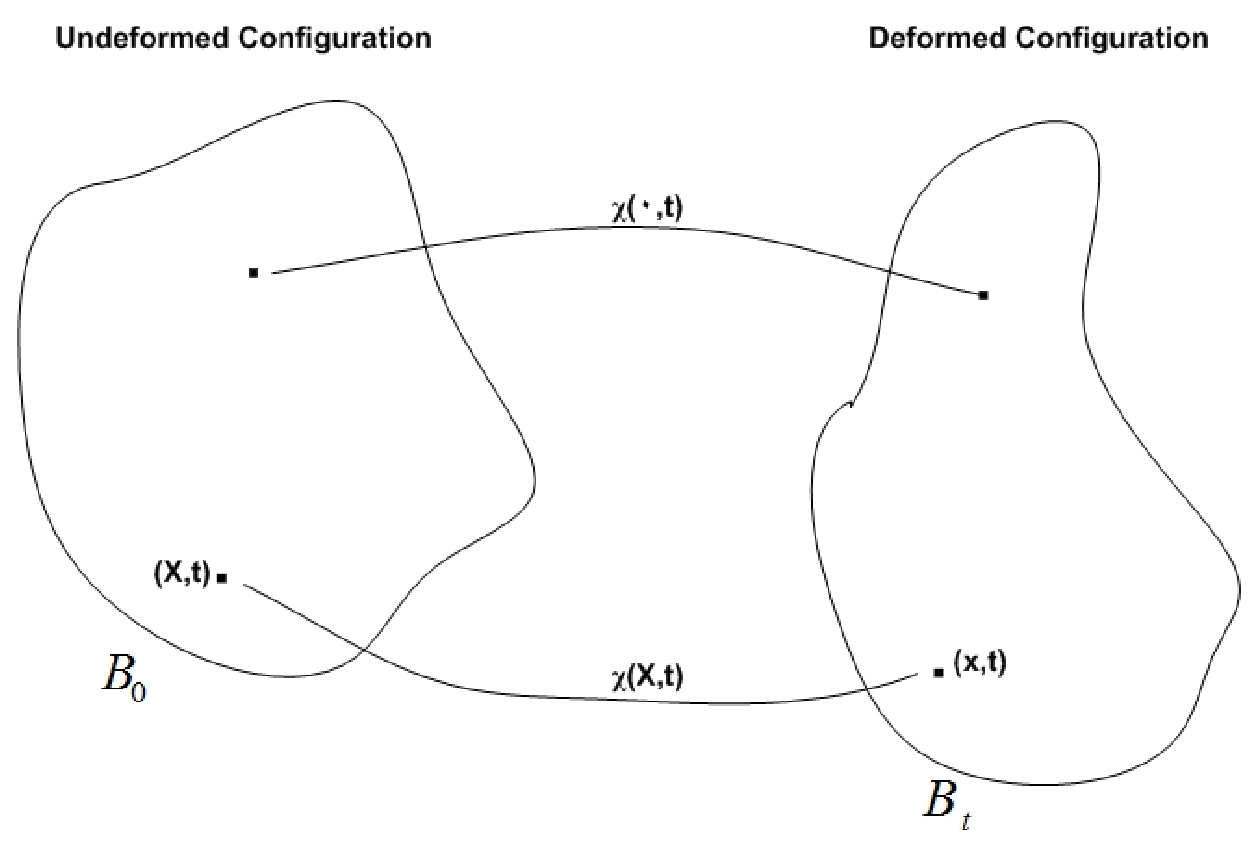
\includegraphics[scale = .5]{config_gragh_marvin.eps}
\end{center}
\end{figure}

We shall adopt the following notations:\\
Capital letters A,B,C\ldots as indices refer to material coordinates: $ X_{A},\  A \in \left\{1,2,3\right\}$\\
Lowercase letters i,j,k\ldots as indices refer to spatial coordinates: $ x_{i},\  i \in \left\{1,2,3\right\}$\\
Eienstein's summation convention:\\
$$ x_{i}x_{i} = x_{1}^2 + x_{2}^2 + x_{3}^2 $$
$$ X_{A}X_{A} = X_{1}^2 + X_{2}^2 + X_{3}^2 $$

\begin{defi}
The \textbf{velocity} of the particle $X$ denoted $\dot x$ is defined by
\begin{equation}
\label{ch1:t1}
 \textbf{v} = \dot x = \frac{\partial \chi(X,t)}{\partial t}
  \end{equation}
\end{defi}

\begin{defi}
The \textbf{acceleration} of the particle $X$ denoted $\ddot x$ is defined by
\begin{equation}
\label{ch1:t2}
\dot \textbf{v} = \ddot x = \frac{\partial^2 \chi(X,t)}{\partial t^2}
\end{equation}
\end{defi}

A quantity can be expressed as a function of either the Lagrangian description $(\textbf{X},t)$ or the Eulerian description $(\textbf{x},t)$.
Changing from one description to the other can be done by using

$$ \Psi(\chi^{-1}(\textbf{x},t),t) = \psi(\textbf{x},t) $$
or
$$ \psi(\chi(\textbf{X},t),t) = \Psi(\textbf{X},t) $$

\begin{defi}
\begin{em} 
The \textbf{alternating tensor}, denoted as $\epsilon_{ABC}$, is defined by 
\begin{equation}
\epsilon_{ABC} = \left\{ 
\begin{array}{l r}
1 & \mbox{if $(A B C)$ is an even permutation of $\{1,2,3\}$}\\
-1 & \mbox{if $(A B C)$ is an odd permutation of $\{1,2,3\}$}\\
0 & \mbox{otherwise}
\end{array}
\right.
\end{equation}  
\end{em}
\end{defi}

\begin{defi}
The \textbf{deformation gradient} denoted $F_{\chi}$ is defined by
\begin{equation}
\label{ch1:t3}
 F_{\chi} = x_{i,A} = \left[\frac{\partial \chi_{i}}{\partial X_{A}}\right] i,A \in \left\{1,2,3\right\}
  \end{equation}
\end{defi}

The deformation gradient of the map $\chi$ is non-singular, since $\chi$ is invertible, and its Jacobian is defined as $J_{\chi} = \mbox{det}F_{\chi}$.

The meaning of $J_{\chi}$  as the change in volume due to the change of coordinates $\chi$ can be easily understood from the following theorem.

\begin{theo}
\begin{em}
Let $dV$ be an infinitesimal domain, given by the triple product $dV = dx^{(1)} \cdot ( dx^{(2)} \times dx^{(3)})$. Also let $dV_{0} = dX^{(1)} \cdot ( dX^{(2)} \times dX^{(3)})$ be the push forward of $dV$, that is $dx^{(i)} = F_{\chi}dX^{(i)}$, for $i\in\left\{1,2,3\right\}$. Then, $$ dV = J_{\chi}dV_{0}.$$
\end{em}
\end{theo}


\textbf{Proof.} $$ dx_{i}^{(\alpha)} = x_{i,A}\ dX_{A}^{(\alpha)} $$
Thus \begin{eqnarray*} \mbox{det}[dx_{i}^{(\alpha)}] &=& \mbox{det}[x_{i,A}\ dX_{A}^{(\alpha)}]\\ \\
&=& \mbox{det}[x_{i,A}]\  \mbox{det}[dX_{A}^{(\alpha)}]\\ \\
&=& J_{\chi} \mbox{det}[dX_{A}^{(\alpha)}]
\end{eqnarray*}
But,
\begin{eqnarray*} \mbox{det}[dx_{i}^{(\alpha)}] &=& \epsilon_{ijk}dx_{i}^{(1)}dx_{j}^{(2)}dx_{k}^{(3)}\\ \\
&=& dx_{i}^{(1)}\epsilon_{ijk} \ dx_{j}^{(2)}dx_{k}^{(3)}\\ \\
&=& dX^{(1)} \cdot ( dX^{(2)} \times dX^{(3)})
\end{eqnarray*}
Therefore,
$$ d\stackrel{\rightarrow}{x} = J_{\chi}d\stackrel{\rightarrow}{X}.$$

which concludes the proof.


\begin{theo}
$$ \frac{DJ_{\chi}}{Dt} = J_{\chi}\mbox{div}(v)$$
\end{theo}

\textbf{Proof.}
$$ J_{\chi} = \mbox{det}[x_{i,A}] = \epsilon_{ABC}\ x_{1,A}\ x_{2,B}\ x_{3,C} $$
Thus
$$ \frac{DJ_{\chi}}{Dt} = \epsilon_{ABC}[(\frac{D}{Dt}x_{1,A})\ x_{2,B}\ x_{3,C} + x_{1,A}\ (\frac{D}{Dt})x_{2,B}\ x_{3,C} + x_{1,A}\ x_{2,B}\ (\frac{D}{Dt})x_{3,C}]$$
But,
\begin{eqnarray*} \frac{D}{Dt}x_{1,A} &=& \frac{\partial^2}{\partial t \partial X_{A}}x_{1}(X,t)\\
&=& \frac{\partial^2}{\partial X_{A} \partial t }x_{1}(X,t)\\ 
&=& \frac{\partial v_{1}}{\partial X_{A}}\\
&=& \frac{\partial v_{1}}{\partial x_{k}} \frac{\partial x_{k}}{\partial X_{A}}\\
&=& v_{i,k} \frac{\partial x_{k}}{\partial X_{A}}
\end{eqnarray*}
Thus 
\begin{eqnarray*} \epsilon_{ABC}(\frac{D}{Dt}x_{1,A}) x_{2,B} x_{3,C} &=& \epsilon_{ABC}v_{1,k}\ x_{k,A}\ x_{2,B}\ x_{3,C}\\
&=& v_{1,1} \epsilon_{ABC}x_{1,A})\ x_{2,B}\ x_{3,C}\\
&=& v_{1,1}J_{\chi}
\end{eqnarray*}
Similarly, 
$$ \epsilon_{ABC} x_{1,A} \ (\frac{D}{Dt})x_{2,B}) x_{3,C} = v_{2,2}J_{\chi} $$
and
$$ \epsilon_{ABC} x_{1,A} x_{2,B} (\frac{D}{Dt})x_{3,C} = v_{3,3}J_{\chi} $$
Thus 
\begin{eqnarray*}\frac{DJ_{\chi}}{Dt} &=& v_{k,k}J_{\chi}\\ 
&=& J_{\chi}\mbox{div}(v)
\end{eqnarray*}




\begin{theo}
Let $V$ be a subset of the deformed configuration, and let $V_{0}$ be a subset of the undeformed configuration. Then for a differentiable function $f$ with continuous partial derivatives, we have
\begin{equation}
\frac{D}{Dt} \int_{V} f(\stackrel{\rightarrow}{x},t)dV = \int_{V}\left\{ {\frac{\partial f}{\partial t} + \nabla\cdot(f\stackrel{\rightarrow}{u})}\right\}dV
\end{equation}
\end{theo}

\textbf{Proof.}
\begin{eqnarray*}
 \frac{D}{Dt} \int_{V} f(\stackrel{\rightarrow}{x},t)dV &=& \frac{D}{Dt} \int_{V_{0}} f(\chi(\textbf{X},t),t)J_{\chi}dV_{0}\\ \\
 &=& \int_{V_{0}}\left\{\frac{Df(\chi(\textbf{X},t),t)}{Dt}J_{\chi} + f(\chi(\textbf{X},t),t)\frac{DJ_{\chi}}{Dt}\right\}dV_{0}\\ \\ 
 &=& \int_{V_{0}}\left\{\frac{Df(\chi(\textbf{X},t),t)}{Dt}J_{\chi} + f(\chi(\textbf{X},t),t)J_{\chi}\nabla v\right\}dV_{0}\\ \\
 &=& \int_{V_{0}}\left\{\frac{Df(\chi(\textbf{X},t),t)}{Dt} + f(\chi(\textbf{X},t),t)\nabla v\right\}J_{\chi}dV_{0}\\ \\
 &=& \int_{V_{0}}\left\{\frac{\partial f(\chi(\textbf{X},t),t)}{\partial t} + v\cdot \nabla f(\chi(\textbf{X},t),t) + f(\chi(\textbf{X},t),t)\cdot \nabla v\right\}J_{\chi}dV_{0}\\ \\
 &=& \int_{V}\left\{\frac{\partial f(\stackrel{\rightarrow}{x},t)}{\partial t} + \mbox{div}(f(\stackrel{\rightarrow}{x},t)v)\right\}dV\\ \\
 \end{eqnarray*}

The Dominated Convergence Theorem is what allows for the passing of the material derivative inside of the integral operator.


\section{Conservation of Mass}


The mass of a fluid $(M_{fluid})$ is given by the integral of the fluid density over the fluid domain i.e. \begin{equation} M_{fluid} = \int_{V} \rho(\stackrel{\rightarrow}{x},t)dV \end{equation}
The Conservation of Mass principle states that the derivative of mass w.r.t time must vanish i.e. \begin{equation} \frac{D}{Dt} \int_{V} \rho(\stackrel{\rightarrow}{x},t)dV = 0. \end{equation}
Applying Reynold's Transport Theorem, we have \begin{equation} \frac{D}{Dt} \int_{V} \rho(\stackrel{\rightarrow}{x},t)dV = \int_{V} \left\{\frac{\partial \rho}{\partial t} + \nabla \cdot(\rho \stackrel{\rightarrow}{u})\right\}dV = 0. \end{equation} Since we are working within the confines of the continuum hypothesis and since this equation must hold true for arbitrarily small domains, we can infer that \begin{equation}\label{cce} \frac{\partial \rho}{\partial t} + \nabla \cdot(\rho \stackrel{\rightarrow}{u}) = 0.\end{equation} which is the continuity equation for compressible flows.

Expanding the divergence term in Eq. (\ref{cce}) yields \begin{equation} \frac{D\rho}{Dt} + \rho \nabla \cdot \stackrel{\rightarrow}{u} = 0. \end{equation} where $\displaystyle{ \frac{D}{Dt} = \frac{\partial}{\partial t} + (\stackrel{\rightarrow}{u}\cdot \nabla)} $

In the case where the density remains constant, Eq.(\ref{cce}) simplifies to \begin{equation}\label{ice} \nabla \cdot \stackrel{\rightarrow}{u} = 0 \end{equation} which is the continuity equation for incompressible flows.

\section{Conservation of Momentum}

The Conservation of Linear Momentum Principle states that the rate of change of momentum w.r.t time is equal to the sum of the acting forces. This is given mathematically by 
\begin{equation}
\frac{D}{Dt}\int_{V} \rho(\stackrel{\rightarrow}{x},t) \stackrel{\rightarrow}{u}dV = \sum \mbox{acting forces}
\end{equation}
 The forces of interest are body forces such as gravity, Coriolis force etc. and surface forces such as pressure and internal friction(viscosity).

Body forces will be expressed as \begin{equation} \int_{V} \rho(\stackrel{\rightarrow}{x},t) g(\stackrel{\rightarrow}{x},t)dV \end{equation} and surface forces will be expressed as \begin{equation} \int_{\partial V} \sigma(\stackrel{\rightarrow}{x},t)\stackrel{\rightarrow}{n}ds \end{equation}
where $\sigma$ is the stress tensor, $\stackrel{\rightarrow}{n}$ is the outward unit normal, and $ \partial V $ is the boundary of the domain $V$

Recasting Newton's 2nd law with the aforementioned information in mind, we have \begin{equation} \frac{D}{Dt} \int_{V} \rho(\stackrel{\rightarrow}{x},t) \stackrel{\rightarrow}{u}dV = \int_{V} \rho(\stackrel{\rightarrow}{x},t) g(\stackrel{\rightarrow}{x},t)dV + \int_{\partial V} \sigma(\stackrel{\rightarrow}{x},t)\stackrel{\rightarrow}{n}ds \end{equation}

Applying Reynold's Transport Theorem to the term on the left yields \begin{equation} \int_{V} \left\{\frac{\partial \rho \stackrel{\rightarrow}{u}}{\partial t} + \nabla \cdot \rho \stackrel{\rightarrow}{u}\stackrel{\rightarrow}{u}\right\}dV = \int_{V} \rho(\stackrel{\rightarrow}{x},t) g(\stackrel{\rightarrow}{x},t)dV + \int_{\partial V} \sigma(\stackrel{\rightarrow}{x},t)\stackrel{\rightarrow}{n}ds \end{equation}
After applying the Divergence Theorem to the last term and regrouping the equation we arrive at \begin{equation} \label{cmom}\frac{\partial \rho \stackrel{\rightarrow}{u}}{\partial t} + (\stackrel{\rightarrow}{u} \cdot \nabla)\rho\stackrel{\rightarrow}{u} + \rho\stackrel{\rightarrow}{u}\nabla \cdot \stackrel{\rightarrow}{u} - \rho \stackrel{\rightarrow}{g} - \nabla \cdot \sigma = 0 \end{equation}

The stress tensor $\sigma$ for viscous fluids is defined as \begin{equation} \sigma := -pI + \tau := -p + \lambda \mbox{div}(\stackrel{\rightarrow}{u})I + 2\mu\delta. \end{equation} Using this stress tensor in Eq. (\ref{cmom}), yields \begin{equation}\label{cmoms} \frac{\partial \rho \stackrel{\rightarrow}{u}}{\partial t} + (\stackrel{\rightarrow}{u} \cdot \nabla)\rho\stackrel{\rightarrow}{u} + \rho\stackrel{\rightarrow}{u}\nabla \cdot \stackrel{\rightarrow}{u} + \mbox{grad}p = (\mu + \lambda)\mbox{grad}(\mbox{div}(\stackrel{\rightarrow}{u})) + \mu\Delta\stackrel{\rightarrow}{u} + \rho\stackrel{\rightarrow}{g} \end{equation}

If the fluid being studied is incompressible(i.e $\rho$ = $\rho_{\infty}$ = constant), Eq. (\ref{cmoms}) reduces to \begin{equation} \label{imom}\frac{\partial \stackrel{\rightarrow}{u}}{\partial t} + (\stackrel{\rightarrow}{u} \cdot \nabla)\ \stackrel{\rightarrow}{u} + \frac{1}{\rho_{\infty}}\mbox{grad}p = \frac{\mu}{\rho_{\infty}}\Delta\stackrel{\rightarrow}{u} + \stackrel{\rightarrow}{g} \end{equation}

Equation (\ref{ice}) together with Eq.(\ref{imom}) comprise what is today known as the Navier-Stokes Equations for incompressible flows.

\section{Dimensional Analysis}

Performing experiments for flow applications can be very expensive and time consuming. Take for example studying the flow of air around automobiles. One would need to build the automobile as well as reproduce the conditions under which they operate. As we know, this is more easily said than done. These kinds of applications motivated the need for prototypes and models. The first step in this process is to nondimensionalize the governing equations. This is done by selecting reference quantities for each of the variable present in the equation. Those variable are $\stackrel{\rightarrow}{u}$,$\stackrel{\rightarrow}{x}$,$p$,and $t$ and the associated reference quantities are $V$,$L$,$\rho_{\infty}V^2$, and $\displaystyle{\frac{L}{V}}$. A quick check will show that these variables and their associated reference quantities are dimensionally homogeneous. Because of this, the dimensionless quantities can be defined as \begin{equation} \stackrel{\rightarrow}{u}^* := \frac{\stackrel{\rightarrow}{u}}{V}, \stackrel{\rightarrow}{x}^* := \frac{\stackrel{\rightarrow}{x}}{L}, p^* := \frac{p}{\rho_{\infty}V^2}, t^* := \frac{Vt}{L} \end{equation}

Recasting equation (15) with these new variable yields, \begin{equation} \frac{V^2}{L}\frac{\partial \stackrel{\rightarrow}{u}^*}{\partial t^*} + \frac{V^2}{L}(\stackrel{\rightarrow}{u}^* \cdot \mbox{grad}^*)\stackrel{\rightarrow}{u}^* + \frac{V^2}{L}\mbox{grad}^* p^* = \frac{V\mu}{L{^2}\rho_{\infty}} \Delta^* \stackrel{\rightarrow}{u}^* + \stackrel{\rightarrow}{g} \end{equation}

Multiplying through by $\displaystyle{\frac{L}{V^2}}$ yields, \begin{equation} \frac{\partial \stackrel{\rightarrow}{u}^*}{\partial t^*} + (\stackrel{\rightarrow}{u}^* \cdot \mbox{grad}^*)\stackrel{\rightarrow}{u}^* + \mbox{grad}^* p^* = \frac{\mu}{L\rho_{\infty}V} \Delta^* \stackrel{\rightarrow}{u}^* + \frac{L}{V^2} \stackrel{\rightarrow}{g} \end{equation}

With the introduction of the dimensionless body force \begin{equation} \stackrel{\rightarrow}{g^{*}} := \frac{L \stackrel{\rightarrow}{g}}{V^2} = \frac{1}{Fr^2}\frac{\stackrel{\rightarrow}{g}}{\left\|\stackrel{\rightarrow}{g}\right\|} \end{equation} the equation becomes \begin{equation} \label{dmome}\frac{\partial \stackrel{\rightarrow}{u}^*}{\partial t^*} + (\stackrel{\rightarrow}{u}^* \cdot \mbox{grad}^*)\stackrel{\rightarrow}{u}^* + \mbox{grad}^* p^* = \frac{\mu}{L\rho_{\infty}V} \Delta^* \stackrel{\rightarrow}{u}^* + \stackrel{\rightarrow}{g^{*}} \end{equation}

The coefficient of the Laplacian gives the reciprocal of the Reynolds number and the last term involves the reciprocal of the square of the Froude number. Recasting Eq. (\ref{dmome}) with this in mind and dropping the * for  convenience yields, \begin{equation} \frac{\partial \stackrel{\rightarrow}{u}}{\partial t} + (\stackrel{\rightarrow}{u} \cdot \mbox{grad})\stackrel{\rightarrow}{u} + \mbox{grad} p = \frac{1}{Re} \Delta \stackrel{\rightarrow}{u} + \stackrel{\rightarrow}{g} \end{equation}

Doing this for the continuity equation will leave it unchanged. It is worth mentioning that the dimensionless quantities that arise in this equation depend heavily on the the reference quantities which usually depend on what is of interest in the flow being analyzed \cite{ffm}. 

\section{Geometries and Boundary Conditions}

As stated previously, the Navier-Stokes Equations are the governing equations for fluid flow. Having this in mind, a question that might arise quite naturally is how does one obtain different flow fields as it relates to various applications. The answer to this question resides in the fact that a specific geometry and various boundary conditions must be supplied when using the Navier-Stokes Equations for a particular application. The boundary conditions that are of particular interest are the Dirichlet boundary condition(no-slip boundary condition), Neumann boundary conditions, mixed boundary conditions, and periodic boundary conditions. Let $\varphi_{n}$ denote the component of velocity orthogonal to the boundary in the exterior normal direction, $\varphi_{t}$ the component of velocity parallel to the boundary in the tangential direction, and $ \displaystyle{\frac{\partial \varphi_{n}}{\partial n}}$ and $ \displaystyle{\frac{\partial \varphi_{t}}{\partial n}}$ be their respective derivatives in the normal direction. 

\subsection{Dirichlet Boundary Condition}

Dirichlet boundary conditions specify the values a solution must take on the boundary of the domain. In the case of fluid flow problems, the no-slip conditions, which are homogeneous Dirichlet boundary conditions, are often enforced on the boundaries of the given geometry. The no-slip condition says that no fluid penetrates the boundary and the fluid is at rest there. Mathematically, this given by \begin{equation} \varphi_{n} = 0, \ \ \ \ \ \  \varphi_{t} = 0 \end{equation} These are to be understood irrespective of the boundary being investigated.

\subsection{Neumann Boundary Condition}

Neumann boundary conditions specify the values that the directional derivative must satisfy along the outward normal to the boundary of the domain. A situation where this occurs is when outflow conditions, which are homogenous Neumann boundary conditions, are supplied. They state that neither velocity component changes in the direction normal to the boundary. Mathematically, this is given by \begin{equation} \frac{\partial \varphi_{n}}{\partial n} = 0, \ \ \ \ \ \ \frac{\partial \varphi_{t}}{\partial n} = 0. \end{equation} The partial derivatives are taken with respect to different axes depending on the orientation of the boundaries.

\subsection{Mixed Boundary Condition}

Mixed boundary conditions are combinations of Dirichlet and Neumann boundary conditions. A situation where this occurs is when free-slip conditions, which are homogeneous mixed boundary conditions, are supplied. They state that no fluid penetrates the boundary and there are no frictional losses at the boundary. Mathematically, this is given by \begin{equation} \varphi_{n} = 0, \ \ \ \ \ \ \frac{\partial \varphi_{t}}{\partial n} = 0 \end{equation}

\subsection{Periodic Boundary Condition}

Periodic boundary conditions occur when the flow problem is periodic over one or more of the coordinate directions. A situation where this occurs is flow over an undulating surface. Since the values on the boundaries are repeated over some period $a$, the computations can be restricted to one period interval.

\section{Conclusion}

In this chapter, we presented the derivation of the Navier-Stokes equations from the conservation of mass and linear momentum. In order to do this, we use Reynold's Transport Theorem. Following the derivation, dimensional analysis of the equations is presented and boundary conditions are discussed so that we have a well-posed problem to work with. In the next chapter, we move from the continuous problem to the discrete problem.
%
%\end{document}
%\documentclass[12pt]{report}
%\setlength{\parindent}{0mm}
%\setlength{\parskip}{14pt}
%\renewcommand{\baselinestretch}{2.0}
%\setlength{\topmargin}{0pt}
%\setlength{\headheight}{0pt}
%\setlength{\headsep}{0pt}
%\setlength{\footskip}{45pt}
%\setlength{\textwidth}{465pt}
%\setlength{\textheight}{660pt}
%\setlength{\oddsidemargin}{10pt}
%\newcommand{\RR}{\mathrm{I\!R\!}}
%\newcommand{\FF}{\mathrm{I\!F\!}}
%\newcommand{\dt}{\frac{\partial}{\partial t}}
%\newcommand{\dq}{\frac{\partial}{\partial q }}
%\newcommand{\dr}{\frac{\partial}{\partial p }}
%\newtheorem{defi}{Definition}[chapter]
%\newtheorem{theo}{Theorem}[chapter]

%\begin{document}

\chapter{Discretization of the Navier-Stokes Equations}

In this chapter, we discuss the finite-differencing scheme for the discretization of the Navier-Stokes equations as well as describe in detail Chorin's Projection Method for solving the resulting Poisson equation for pressure.

\section{Finite Difference Approximations}

\subsection{First Order Finite Difference Approximations}

In order to work efficiently with the series that follow, we introduce the concept of the Big-O notation.

\begin{defi}
Let $f(x)$ and $g(x)$ be two functions defined on a subset of real numbers. We say that $f(x)$ is \textbf{Big-O} of $g(x)$  if there exist positive real numbers $C$ and $x_{0}$ such that 
$$ \left|f(x)\right| \leq C\left|g(x)\right| \ \forall x > x_{0} $$

This can also be formulated to study the behavior of $f(x)$ near some real number $a$ as follows: Let $f(x)$ and $g(x)$ be two functions defined on a subset of real numbers. We say that $f(x)$ is \textbf{Big-O} of $g(x)$  if there exist positive real numbers $C$ and $\delta$ such that

$$ \left|f(x)\right| \leq C\left|g(x)\right| for \left|x-a\right| < \delta $$

\end{defi}

In order to perform the discretization of the governing equation for fluid motion, one must be able to approximate the continuous differential operator at a finite number of grid points. 
Consider a function $u(x,t)$ with $ x \in [0,L]$ and $ t \in [0,T]$. A discretization of the function $u$ is obtained by considering only
the values $u_{i}^{j}$ at a finite number of grid points $(x_{i},t_{j})$. Applying Taylor�s series expansion to $u(x_{i},t_{j}+\delta t)$ gives \begin{equation} u(x_{i},t_{j}+\delta t) = u(x_{i},t_{j}) + u_{t}(x_{i},t_{j}) \delta t + u_{tt}(x_{i},t_{j}) \frac{(\delta t)^2}{2} + u_{ttt}(x_{i},t_{j}) \frac{(\delta t)^3}{3!} + O((\delta t)^4) \end{equation} The following convention will be used in an effort to reduce the use of notation throughout this work. \begin{equation} u_{i}^{j} = u(x_{i},t_{j}) = u(i\delta x, j\delta t)\  i =0,1,\cdots ,m; \ j = 0,1,\cdots .n. \end{equation} Recasting the above equation with this in mind yields \begin{equation} \label{ffd}u_{i}^{j+1} = u_{i}^{j} + (u_{t})_{i}^{j} \delta t + (u_{tt})_{i}^{j} \frac{(\delta t)^2}{2} + (u_{ttt})_{i}^{j} \frac{(\delta t)^3}{3!} + O((\delta t)^4). \end{equation} Truncating this equation at the second order term and solving for $(u_{t})_{i}^{j}$ yields \begin{equation}  (u_{t})_{i}^{j} = \frac{u_{i}^{j+1} - u_{i}^{j}}{\delta t} + O(\delta t). \end{equation} Therefore \begin{equation} (u_{t})_{i}^{j} \approx \frac{u_{i}^{j+1} - u_{i}^{j}}{\delta t} \end{equation}
This equation is known as the two point forward finite difference approximation of $\displaystyle{\frac{\partial u}{\partial t}}.$ 

Applying Taylor�s series expansion to $u_{i}^{j-1}$ gives \begin{equation}\label{bfd} u_{i}^{j-1} = u_{i}^{j} - (u_{t})_{i}^{j} \delta t + (u_{tt})_{i}^{j} \frac{(\delta t)^2}{2} - (u_{ttt})_{i}^{j} \frac{(\delta t)^3}{3!} + O((\delta t)^4) \end{equation}

Truncating this equation at the second order term and solving for $(u_{t})_{i}^{j}$ yields \begin{equation}  (u_{t})_{i}^{j} = \frac{u_{i}^{j} - u_{i}^{j-1}}{\delta t} + O(\delta t). \end{equation} Therefore \begin{equation} (u_{t})_{i}^{j} \approx \frac{u_{i}^{j} - u_{i}^{j-1}}{\delta t} \end{equation}
 This equation is known as the two point backward finite difference approximation of $\displaystyle{\frac{\partial u}{\partial t}}.$

Doing the difference of equations (ffd) and (bfd) yield \begin{equation} u_{i}^{j+1} - u_{i}^{j-1} = 2(u_{t})_{i}^{j} \delta t + O((\delta t)^3). \end{equation} Solving for $(u_{t})_{i}^{j}$ yields \begin{equation} (u_{t})_{i}^{j} = \frac{u_{i}^{j+1} - u_{i}^{j-1}}{2\delta t} + O((\delta t)^2). \end{equation} Therefore \begin{equation} (u_{t})_{i}^{j} \approx \frac{u_{i}^{j+1} - u_{i}^{j-1}}{2\delta t} \end{equation} This equation is known as the two point central difference approximation of $\displaystyle{\frac{\partial u}{\partial t}}.$

The forward and backward finite difference approximation of $\displaystyle{\frac{\partial u}{\partial t}}.$ have an error of order $\delta t$ where as the central finite difference approximation of $\displaystyle{\frac{\partial u}{\partial t}}.$ has an error of order $(\delta t)^2$ which indicates that for most applications, the central finite difference approximation will yield more accurate results. All of the finite difference approximations for the spatial derivatives can be found in an analogous way to the difference approximations found for the time derivative.

\subsection{Higher Order Finite Difference Approximations}

Following a similar procedure to that used in the previous section, higher order finite difference approximations can be derived but only the second order central finite difference approximations will be investigated here.

To accomplish this, the Taylor Series Expansion is again found for $u_{i}^{j+1}$ and $u_{i}^{j-1}$. 

\begin{equation} u_{i}^{j-1} = u_{i}^{j} - (u_{t})_{i}^{j} \delta t + (u_{tt})_{i}^{j} \frac{(\delta t)^2}{2} - (u_{ttt})_{i}^{j} \frac{(\delta t)^3}{3!} + O((\delta t)^4) \end{equation}

\begin{equation} u_{i}^{j+1} = u_{i}^{j} + (u_{t})_{i}^{j} \delta t + (u_{tt})_{i}^{j} \frac{(\delta t)^2}{2} + (u_{ttt})_{i}^{j} \frac{(\delta t)^3}{3!} + O((\delta t)^4). \end{equation}

Taking the sum of these expansions yields
\begin{equation} u_{i}^{j-1} + u_{i}^{j+1} = 2u_{i}^{j} + (u_{tt})_{i}^{j}(\delta t)^2 + O((\delta t)^4) \end{equation}

Therefore, \begin{equation} (u_{tt})_{i}^{j} \approx \frac{u_{i}^{j-1}-2u_{i}^{j}+u_{i}^{j+1}}{(\delta t)^2} \end{equation}
 
This equation is known as the three point central difference approximation of $\displaystyle{\frac{\partial^2 u}{\partial t^2}}.$

The second order forward and backward finite difference approximations can be found by composing any of the first order approximations.

When dealing with Navier-Stokes equations, using a purely finite-difference discretization would lead to stability issues. We introduce the Donor-Cell discretization scheme in order to circumvent this stability issue. 

\section{The Donor-Cell Discretization Scheme}

We define the donor-cell discretization \cite{nsfd} of some convective term $\displaystyle{\frac{d(ku)}{dx}}$ by

\begin{equation}
\left[\frac{d(ku)}{dx}\right]_{i}^{dc} := \frac{k_{r}u_{r} - k_{l}u_{l}}{\delta x}
\end{equation}

where $u_r$ and $u_l$ are chosen based on the sign of $k_r$ and $k_l$, i.e.

$$ u_r := \left \{
\begin{array}{l r}
u_i & k_r > 0\\
u_{i+1} & k_r < 0
\end{array}
\right. \hspace{1in}
u_l := \left \{
\begin{array}{l r}
u_{i-1} & k_l > 0\\
u_{i} & k_l < 0
\end{array}
\right.$$

In order to avoid these case distinction, the donor-cell discretization can written as

\begin{equation}
\left[\frac{d(ku)}{dx}\right]_{i}^{dc} := \frac{1}{2\delta x}\left(k_{r}(u_{i} + u_{i+1}) - k_{l} (u_{i-1} + u_{i}) + \left|k_{r}\right|(u_{i} - u_{i+1}) - \left|k_{l}\right|(u_{i-1} - u_{i})\right)
\end{equation}

The need for this scheme will be explained in the sections covering the discretization of the Navier-Stokes equations.

\section{Discretization of the Heat Equation}

In this subsection, we introduce the finite difference approximation of the one-dimensional heat equation without sources on a finite interval $0<x<L$. Handling of the initial and boundary conditions will be ignored here and will be dealt with in detail for the Navier-Stokes Equations. The Heat Equation as specified is given by

\begin{eqnarray*}
\left \{
\begin{array}{l r}
\displaystyle{\frac{\partial u}{\partial t} = k\frac{\partial^2 u}{\partial x^2}}\\
 u(0,t)=0 & \\
u(L,t)=0 & \\
u(x,0)=f(x) & 
\end{array}
\right. 
\end{eqnarray*}

In order to discretize this equation, we replace the time derivative with its forward finite difference approximation and the space derivative with its central finite difference approximation yielding \begin{equation} \frac{u_{i}^{j+1} - u_{i}^{j}}{\Delta t} = k\frac{u_{i-1}^{j} -2u_{i}^{j} + u_{i+1}^{j}}{(\Delta x)^2}. \end{equation} The forward finite difference approximation was used for the time derivative because of the initial condition supplied and the central finite difference approximation was used for the space derivative because of the boundary conditions supplied. Since the truncated terms go to zero as $\Delta t$ and $\Delta x$ go to zero, the numerical approximate is said to be  \textbf{consistent} with the given PDE in its continuous form. The analysis for Navier-Stokes equations are now investigated.

\section{Discretization of the Spatial Derivative}

We use a staggered grid in order to discretize the Navier-Stokes Equations \cite{nsfd}. In this approach, the horizontal velocities $u$ are located at the midpoint of the vertical cell edges, the vertical velocities $v$ are located at the midpoint of the horizontal cell edges, and the pressure $p$ is located at the cell centers. Using the staggered grid approach eliminates the pressure oscillations that would occur with a grid in which $u$,$v$,and $p$ are all located at the same grid point.
\begin{figure}
\begin{center}
\caption{Staggered Grid}
\label{sg}
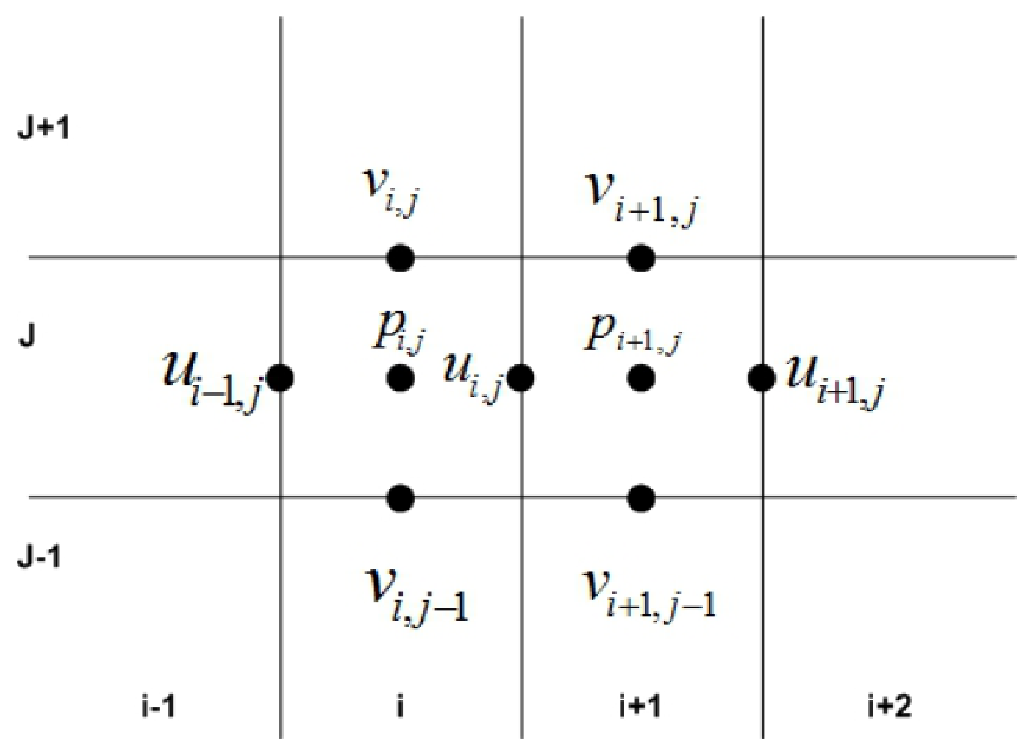
\includegraphics[scale = .5]{staggered_grid_marvin.eps}
\end{center}
\end{figure}
In order to discretize the continuity equation, we replace the spatial derivatives $\displaystyle{\frac{\partial u}{\partial x}}$ and $\displaystyle{\frac{\partial v}{\partial y}}$ by centered differences with half the mesh width. That is, 

\begin{equation}
\left[\frac{\partial u}{\partial x}\right]_{i}^{j} := \frac{u_{i}^{j} - u_{i-1}^{j}}{\delta x} \hspace{1in} \left[\frac{\partial v}{\partial y}\right]_{i}^{j} := \frac{v_{i}^{j} - v_{i}^{j-1}}{\delta y}
\end{equation}

The terms $\displaystyle{\frac{\partial^2 u}{\partial x^2}}$, $\displaystyle{\frac{\partial^2 u}{\partial y^2}}$,$\displaystyle{\frac{\partial^2 v}{\partial x^2}}$, and $\displaystyle{\frac{\partial^2 v}{\partial y^2}}$ in the momentum equation are replaced with the second order centered difference approximations as discussed earlier in the chapter. These terms form the so called diffusive terms of the momentum equations. The remaining terms present small complications due to the form of the grid spacing that was chosen. For the terms, $\displaystyle{\frac{\partial uv}{\partial y}}$ and $\displaystyle{\frac{\partial u^2}{\partial x}}$ we use the averages of \textbf{u},\textbf{v} and \textbf{u} respectively to obtain suitable values of the product lying in the two vertical directions. 
That is,

\begin{equation}
\left[\frac{\partial (uv)}{\partial y}\right]_{i}^{j} := \frac{1}{\delta y}\left(\frac{(v_{i}^{j} + v_{i+1}^{j})}{2} \frac{(u_{i}^{j} + u_{i}^{j+1})}{2} - \frac{(v_{i}^{j-1} + v_{i+1}^{j-1})}{2} \frac{(u_{i}^{j-1} + u_{i}^{j})}{2}\right)
\end{equation}

and

\begin{equation}
\left[\frac{\partial (u^2)}{\partial x}\right]_{i}^{j} := \frac{1}{\delta x}\left(\left(\frac{u_{i}^{j} + u_{i+1}^{j}}{2}\right)^2 - \left(\frac{u_{i-1}^{j} + u_{i}^{j}}{2}\right)^2\right)
\end{equation}

The terms $\displaystyle{\frac{\partial (uv)}{\partial x}}$ and $\displaystyle{\frac{\partial (u^2)}{\partial x}}$ are treated in an analogous fashion. Since at high Reynolds numbers the convective terms in our equation become dominant and may present problems with stability, a blend of the central differences and the donor-cell discretization is used. This leads to the following discretization.

\begin{eqnarray*} \left[\frac{\partial (u^2)}{\partial x}\right]_{i}^{j} := \frac{1}{\delta x}\left(\left(\frac{u_{i}^{j} + u_{i+1}^{j}}{2}\right)^2 - \left(\frac{u_{i-1}^{j} + u_{i}^{j}}{2}\right)^2\right)& &
& & + \gamma \frac{1}{\delta x} \left(\frac{\left|u_{i}^{j} + u_{i+1}^{j}\right|}{2}\frac{(u_{i}^{j} - u_{i+1}^{j})}{2} - \frac{\left|u_{i-1}^{j} + u_{i}^{j}\right|}{2}\frac{(u_{i-1}^{j} - u_{i}^{j})}{2}\right) \end{eqnarray*}

\begin{eqnarray*} \left[\frac{\partial (uv)}{\partial y}\right]_{i}^{j} := \frac{1}{\delta y}\left(\frac{(v_{i}^{j} + v_{i+1}^{j})}{2} \frac{(u_{i}^{j} + u_{i}^{j+1})}{2} - \frac{(v_{i}^{j-1} + v_{i+1}^{j-1})}{2} \frac{(u_{i}^{j-1} + u_{i}^{j})}{2}\right)& &
& & + \gamma \frac{1}{\delta y} \left(\frac{\left|v_{i}^{j} + v_{i+1}^{j}\right|}{2}\frac{(u_{i}^{j} - u_{i}^{j+1})}{2} - \frac{\left|v_{i}^{j-1} + v_{i+1}^{j-1}\right|}{2}\frac{(u_{i}^{j-1} - u_{i}^{j})}{2}\right) \end{eqnarray*}

$$ \left[\frac{\partial^2 u}{\partial x^2}\right]_{i}^{j} :=  \frac{u_{i+1}^{j} - 2u_{i}^{j} + u_{i-1}^{j}}{(\delta x)^2} $$

$$ \left[\frac{\partial^2 u}{\partial y^2}\right]_{i}^{j} :=  \frac{u_{i}^{j+1} - 2u_{i}^{j} + u_{i}^{j-1}}{(\delta y)^2} $$

$$ \left[\frac{\partial p}{\partial x}\right]_{i}^{j} :=  \frac{p_{i+1}^{j} - p_{i}^{j} }{(\delta x)} $$


\begin{eqnarray*} \left[\frac{\partial (v^2)}{\partial y}\right]_{i}^{j} := \frac{1}{\delta y}\left(\left(\frac{v_{i}^{j} + v_{i}^{j+1}}{2}\right)^2 - \left(\frac{v_{i}^{j-1} + v_{i}^{j}}{2}\right)^2\right)& &
& & + \gamma \frac{1}{\delta y} \left(\frac{\left|v_{i}^{j} + v_{i}^{j+1}\right|}{2}\frac{(v_{i}^{j} - u_{i}^{j+1})}{2} - \frac{\left|v_{i}^{j-1} + v_{i}^{j}\right|}{2}\frac{(v_{i}^{j-1} - v_{i}^{j})}{2}\right) \end{eqnarray*}

\begin{eqnarray*} \left[\frac{\partial (uv)}{\partial x}\right]_{i}^{j} := \frac{1}{\delta x}\left(\frac{(u_{i}^{j} + u_{i}^{j+1})}{2} \frac{(v_{i}^{j} + v_{i+1}^{j})}{2} - \frac{(u_{i-1}^{j} + u_{i-1}^{j+1})}{2} \frac{(v_{i-1}^{j} + v_{i}^{j})}{2}\right) & &
& & + \gamma \frac{1}{\delta x} \left(\frac{\left|u_{i}^{j} + u_{i}^{j+1}\right|}{2}\frac{(v_{i}^{j} - v_{i+1}^{j})}{2} - \frac{\left|u_{i-1}^{j} + u_{i-1}^{j+1}\right|}{2}\frac{(v_{i-1}^{j} - v_{i}^{j})}{2}\right) \end{eqnarray*}

$$ \left[\frac{\partial^2 v}{\partial x^2}\right]_{i}^{j} :=  \frac{v_{i+1}^{j} - 2v_{i}^{j} + v_{i-1}^{j}}{(\delta x)^2} $$

$$ \left[\frac{\partial^2 v}{\partial y^2}\right]_{i}^{j} :=  \frac{v_{i}^{j+1} - 2v_{i}^{j} + v_{i}^{j-1}}{(\delta y)^2} $$

$$ \left[\frac{\partial p}{\partial y}\right]_{i}^{j} :=  \frac{p_{i}^{j+1} - p_{i}^{j} }{(\delta y)} $$

The parameter $\gamma$ lies between 0 and 1 and should be chosen such that

$$ \displaystyle{\gamma \geq \max_{i,j} \left(\left|\frac{u_{i,j}\delta t}{\delta x}\right|,\left|\frac{v_{i,j}\delta t}{\delta y}\right|\right)} $$

Appropriately discretized boundary conditions must also be supplied depending on the nature of the problem being studied. 

\section{Discretization of the Time Derivative}

In order to discretize the time derivatives occurring in the momentum equations, first order finite differences are used \cite{nsfd}.  Doing this yields

\begin{equation}
\left[\frac{\partial u}{\partial t}\right]^{(n+1)} := \frac{u^{(n+1)} - u^{(n)}}{\delta t}, \hspace{1in} \left[\frac{\partial v}{\partial t}\right]^{(n+1)} := \frac{v^{(n+1)} - v^{(n)}}{\delta t}
\end{equation} 

\subsection{The Time-Stepping Algorithm}

The time-stepping algorithm begins by discretizing the time derivatives appearing in the momentum equation. As a result, we have

\begin{equation}
u^{(n+1)} = u^{(n)} + \delta t\left[\frac{1}{Re}\left(\frac{\partial^2 u}{\partial x^2} + \frac{\partial^2 u}{\partial y^2}\right) - \frac{\partial (u^2)}{\partial x} - \frac{\partial (uv)}{\partial y} + g_{x} - \frac{\partial p}{\partial x}\right]
\end{equation}

\begin{equation}
v^{(n+1)} = v^{(n)} + \delta t\left[\frac{1}{Re}\left(\frac{\partial^2 v}{\partial x^2} + \frac{\partial^2 v}{\partial y^2}\right) - \frac{\partial (uv)}{\partial x} - \frac{\partial (v^2)}{\partial y} + g_{y} - \frac{\partial p}{\partial y}\right]
\end{equation}

We introduce the abbreviations 

\begin{equation}
F := u^{(n)} + \delta t\left[\frac{1}{Re}\left(\frac{\partial^2 u}{\partial x^2} + \frac{\partial^2 u}{\partial y^2}\right) - \frac{\partial (u^2)}{\partial x} - \frac{\partial (uv)}{\partial y} + g_{x} - \frac{\partial p}{\partial x}\right]
\end{equation}

\begin{equation}
G := v^{(n)} + \delta t\left[\frac{1}{Re}\left(\frac{\partial^2 v}{\partial x^2} + \frac{\partial^2 v}{\partial y^2}\right) - \frac{\partial (uv)}{\partial x} - \frac{\partial (v^2)}{\partial y} + g_{y} - \frac{\partial p}{\partial y}\right]
\end{equation}

and associate to them the time level $n$ to arrive at

\begin{equation} \label{nvfp}
u^{(n+1)} = F^{(n)} - \delta t \frac{\partial p}{\partial x} \hspace{1in} v^{(n+1)} = G^{(n)} - \delta t \frac{\partial p}{\partial y}
\end{equation}

We associate the time level $(n+1)$ to the pressure term yielding

\begin{equation}
u^{(n+1)} = F^{(n)} - \delta t \frac{\partial p^{(n+1)}}{\partial x} \hspace{1in} v^{(n+1)} = G^{(n)} - \delta t \frac{\partial p^{(n+1)}}{\partial y}
\end{equation}

Upon substituting this equation into the continuity equation, we obtain,

\begin{equation}
\frac{\partial u^{(n+1)}}{\partial x} + \frac{\partial v^{(n+1)}}{\partial y} = \frac{\partial F^{(n)}}{\partial x} - \delta t \frac{\partial^2 p^{(n+1)}}{\partial x^2} + \frac{\partial G^{(n)}}{\partial y} - \delta t \frac{\partial^2 p^{(n+1)}}{\partial y^2} = 0
\end{equation}

Therefore,

\begin{equation}
\frac{\partial^2 p^{(n+1)}}{\partial x^2} + \frac{\partial^2 p^{(n+1)}}{\partial y^2} = \frac{1}{\delta t} \left(\frac{\partial F^{(n)}}{\partial x} + \frac{\partial G^{(n)}}{\partial y}\right)
\end{equation}

which is a Poisson equation for pressure \cite{nsfd}.

In order to solve this resulting Poisson equation, boundary values for the pressure are required. These result from multiplying the time-discrete momentum equation with the exterior unit normal $\stackrel{\rightarrow}{n} := (n_{1},n_{2})^{T}$ on the boundary yielding,

\begin{eqnarray*}
\mbox{grad} p^{(n+1)} \cdot \stackrel{\rightarrow}{n} &=& \frac{\partial p^{(n+1)}}{\partial x}n_{1} + \frac{\partial p^{(n+1)}}{\partial y}n_{2}\\
																											&=& -\frac{1}{\delta t}\left((u^{(n+1)} - F^{(n)})n_{1} + (v^{(n+1)} - G^{(n)})n_{2}\right)
\end{eqnarray*}

Discretization of the Poisson equation will result in a linear system of equation. Because of the computational cost that arises using elementary methods for solving this system such as Guassian Elimination, a technique known as as Successive Over Relaxation(SOR) \cite{ncse} is used . Successive Over Relaxation is a generalization of the more familiar Guass-Seidel and Jacobi Method.

The above approach is known as Chorin projection method and is attributed to Alexandre Joel Chorin \cite{cpm}.

In order to get the fully discretized momentum equations, we take the time-discretized momentum equations and associate to the spatial derivatives their corresponding spatial discretizations. 
Doing so yields,

\begin{equation}
\overline{\overline{u}}_{i}^{j} = \overline{F}_{i}^{j} - \frac{\delta t}{\delta x}(\overline{\overline{p}}_{i+1}^{j} - \overline{\overline{p}}_{i}^{j})
\end{equation}

\begin{equation}
\overline{\overline{v}}_{i}^{j} = \overline{G}_{i}^{j} - \frac{\delta t}{\delta y}(\overline{\overline{p}}_{i}^{j+1} - \overline{\overline{p}}_{i}^{j})
\end{equation}

where $\overline{\overline{u}}$ stands for $u$ with associated time level $(n+1)$, and $\overline{u}$ stands for $u$ with associated time level $(n)$.

In order to maintain stability of the presented algorithm, the time step $\delta t$ is chosen such that the following conditions hold.

\begin{equation}
\frac{2\delta t}{Re} < \left(\frac{1}{\delta x^2} + \frac{1}{\delta y^2}\right)^{-1},\ \ \ \  \left|u_{max}\right|\delta t < \delta x,\ \ \ \  \left|v_{max}\right|\delta t < \delta y
\end{equation}

The latter two of these conditions are known as the famous Courant-Friedrichs-Lewy(CFL) conditions. They state that a fluid particle cannot, in any given time step, travel a distance greater than the grid spacing.
Choosing $\delta t$ to be the minimal for these conditions guarantees stability of the algorithm, i.e.

\begin{equation}
\delta t := \tau \min\left(\frac{Re}{2}\left(\frac{1}{\delta x^2} + \frac{1}{\delta y^2}\right)^{-1},\frac{\delta x}{\left|u_{max}\right|},\frac{\delta y}{\left|v_{max}\right|}\right)
\end{equation}
 
where $\tau \in [0,1]$ is a safety factor.
 
\section{Conclusion}

In this chapter, we presented the discretization of the Navier-Stokes equations using the finite-differencing technique. Various finite-difference approximations of the derivatives appearing in our equation were derived as well as the Donor-Cell discretiztion technique for handling stability issues that arise when dealing with the discretization of the convective terms of the Navier-Stokes equations. From this point, Chorin Projection method was presented to enforce the incompressibility condition. In the next chapter, we present the functions needed to implement the algorithm discussed in this chapter. 
 
%\end{document}


%\documentclass[12pt]{report}
%\setlength{\parindent}{0mm}
%\setlength{\parskip}{14pt}
%\renewcommand{\baselinestretch}{2.0}
%\setlength{\topmargin}{0pt}
%\setlength{\headheight}{0pt}
%\setlength{\headsep}{0pt}
%\setlength{\footskip}{45pt}
%\setlength{\textwidth}{465pt}
%\setlength{\textheight}{660pt}
%\setlength{\oddsidemargin}{10pt}
%\newcommand{\RR}{\mathrm{I\!R\!}}
%\newcommand{\FF}{\mathrm{I\!F\!}}
%\newcommand{\dt}{\frac{\partial}{\partial t}}
%\newcommand{\dq}{\frac{\partial}{\partial q }}
%\newcommand{\dr}{\frac{\partial}{\partial p }}
%\newtheorem{defi}{Definition}[chapter]
%\newtheorem{theo}{Theorem}[chapter]

%\begin{document}

\chapter{Implementation of the Navier-Stokes Equations Solver}

In this chapter, we discuss the functions needed to implement the algorithm for finding the numerical solutions to Navier-Stokes equations. All these functions were implemented in 
C by Griebel {\em et al}.\cite{nsfd}. The program is available as an open source software called Nast2d.  

\section{The Program}

The following is an explaination of the input paramaters and functions used in the aforementioned open source code.
\begin{itemize}
\item \texttt{inputfile} is the inputfile name
\item \texttt{problem} is the specific predefined problem types
\item \texttt{xlength} is the length of the computational domain in the x direction
\item \texttt{ylength} is the length of the computational domain in the y direction
\item \texttt{imax} is the number of subinterval of xlength
\item \texttt{jmax }is the number of subinterval of ylength
\item \texttt{delx} is the spatial step size in the x direction
\item \texttt{dely} is the spatial step size in the y direction
\item \texttt{delt} is the time step size
\item \texttt{$t_{end}$} is the final time level
\item \texttt{tau} is a safety factor used when choosing the time step
\item \texttt{itermax} is the maximum number of iterations
\item \texttt{eps} is the stopping tolerance for the pressure iteration
\item \texttt{omg} successive overrelaxation parameter
\item \texttt{gamma} is the parameter chosen to maintain stability for convective terms
\item \texttt{Re} is the Reynold's number
\item \texttt{GX} is the body force in the x direction
\item \texttt{GY} is the body force in the y direction
\item \texttt{UI} is the initial velocity in the horizontal direction
\item \texttt{VI} is the initial velocity in the vertical direction
\item \texttt{PI} is the initial pressure
\item \texttt{wW }is the western boundary
\item \texttt{wE} is the eastern boundary
\item \texttt{wN} is the northern boundary
\item \texttt{wS} is the southern boundary
\end{itemize}

Using the described variables, the following functions are used to implement the algorithm.

\begin{itemize}
	
	\item \texttt{ReadParameter}( inputfile, problem, xlength, ylength, imax, jmax, delx, dely, delt, $t_{end}$, tau, itermax, eps, omg, gamma, Re, GX, GY, UI, VI, PI, wW, wE, wN, wS ) 

This function is tasked with reading all of the input parameters required for the program.

	\item \texttt{InitUVP}( U, V, P, imax, jmax, UI, VI, PI)

This function is tasked with initializing the arrays $U$, $V$, and $P$ with their corresponding inital values $UI$, $VI$, and $PI$.

	\item \texttt{CompDelt}( delt, imax, jmax, delx, dely, U, V, Re, tau)
	
This function is tasked with calculating the stepsize delt for the next time step according to equation(). If tau < 0, the stepsize read in from ReadParameter is to be used.

	\item \texttt{SetBCond}( U, V, imax, jamx, wW, wE, wN, wS)
	
This function is tasked with setting the boundary data parameters wW, wE, wN, wS for the arrays U and V.

	\item \texttt{SetSPECBcond}( U, V, imax, jamx, wW, wE, wN, wS)
	
This function is tasked with specifying problem specific boundary conditions. 

	\item \texttt{CompFG}( U, V, F, G, imax, jamx, delt, delx, dely, GX, GY, gamma, Re)
	
This function is tasked with the computation of $F$ and $G$ according to equation().

	\item \texttt{CompRHS}( F, G, RHS, imax, jmax, delt, delx, dely) 
	
This function is tasked with the computation of the right-hand side of the pressure equation.

	\item \texttt{Poisson}( P, RHS, imax, jmax, delx, dely, eps, itermax, omg, res)
	
This function is tasked with performing the successive over relaxation iteration for the pressure Poisson equation and is terminated once the residual norm reaches its tolerance eps, or once the maximum number of iterations(itermax) is reached.

	\item \texttt{AdapUV}( U, V, F, G, P, imax, jmax, delt, delx, dely)
	
This function is tasked with calculating the new velocities according to Eq. (\ref{nvfp}).
	
\end{itemize} 


\section{Conclusion}

In this chapter, we presented the functions needed for implementation of the aformentioned algorithm. In the next chapter, techniques to visualize the numerical solutions obtained are presented.
%\end{document}
%\documentclass[12pt]{report}
%\setlength{\parindent}{0mm}
%\setlength{\parskip}{14pt}
%\renewcommand{\baselinestretch}{2.0}
%\setlength{\topmargin}{0pt}
%\setlength{\headheight}{0pt}
%\setlength{\headsep}{0pt}
%\setlength{\footskip}{45pt}
%\setlength{\textwidth}{465pt}
%\setlength{\textheight}{660pt}
%\setlength{\oddsidemargin}{10pt}
%\newcommand{\RR}{\mathrm{I\!R\!}}
%\newcommand{\FF}{\mathrm{I\!F\!}}
%\newcommand{\dt}{\frac{\partial}{\partial t}}
%\newcommand{\dq}{\frac{\partial}{\partial q }}
%\newcommand{\dr}{\frac{\partial}{\partial p }}
%\newtheorem{defi}{Definition}[chapter]
%\newtheorem{theo}{Theorem}[chapter]

%\begin{document}

\chapter{Visualization Techniques}

Being able to visualize the results obtained from the implemented algorithm discussed in the previous chapter is a very important part of the analysis process. When dealing with fluid flow problems, having visual data can go a long way in interpreting numerical results. In this chapter, we discuss some visualization techniques that can be used when working with the Navier-Stokes equations.

\section{Vector Field Representation}

A 2-D vector field can be used to visualize various flow field problems. It can be visualized as arrows, with a given magnitude and direction, attached to each point in the plane. The vectors are drawn by taking the corresponding vector values for the horizontal velocity u and the vertical velocity v and finding their geometric sum.
\section{Streamlines}

\begin{defi}
A \textbf{streamline} is a line whose tangent at each point is in the direction of the velocity vector at that point. These plots appear as contour graphs once visualized. 
\end{defi}

\section{Conclusion}
In this chapter, we investigated two ways to visualize the numerical solutions of the Navier-Stokes equations. Open source Matlab programs were used for the visualization. Other commercial as well as non-commercial visualization softwares are availible for use depending on the abilitiy of the user and results desired. In the chapter to follow, we use these visualization techniques to present different fluid flow problems.
%\end{document}
%\documentclass[12pt]{report}
%\usepackage{graphicx}
%\setlength{\parindent}{0mm}
%\setlength{\parskip}{14pt}
%\renewcommand{\baselinestretch}{2.0}
%\setlength{\topmargin}{0pt}
%\setlength{\headheight}{0pt}
%\setlength{\headsep}{0pt}
%\setlength{\footskip}{45pt}
%\setlength{\textwidth}{465pt}
%\setlength{\textheight}{660pt}
%\setlength{\oddsidemargin}{10pt}
%\newcommand{\RR}{\mathrm{I\!R\!}}
%\newcommand{\FF}{\mathrm{I\!F\!}}
%\newcommand{\dt}{\frac{\partial}{\partial t}}
%\newcommand{\dq}{\frac{\partial}{\partial q }}
%\newcommand{\dr}{\frac{\partial}{\partial p }}
%\newtheorem{defi}{Definition}[chapter]
%\newtheorem{theo}{Theorem}[chapter]


%\begin{document}

\chapter{Examination of Classical Flows}

\section{Flow Over a Flat Plate}

Using a similarity transform, we look for a stream function $\psi(x,y)$ in the form 
$$\psi(x,y) = \sqrt{(\nu U_0 x)}f(\eta)\ \ \ \ \ \eta = y \sqrt{\frac{U_0}{\eta x}}.$$

After simplification, we arrive at $$f'''(\eta) + \frac{1}{2}f(\eta)f''(\eta) = 0$$
which is Blasius equation. It is subject to the boundary conditions 
$$ y=0: V_x = 0 \ \ \  \eta = 0, f'(0) = 0$$
$$ y=0: V_y = 0 \ \ \  \eta = 0, f(0) = 0$$
$$ y=\infty: V_x = U_0 \ \ \  \eta = 0, f'(\infty) = 1.$$
The friction on the lower plate is proportional to $f''(0) \approx 0.332$. In order to confirm this result using Nast2d, we simulated a flow over a flat plate as follows.  
We solve the 2-D Navier-Stokes equation until we reach steady state. We used the following physical parameters. The length of the plate was chosen to be $30$ and the inflow velocity is $U_0 = 1$. The Reynolds number for the flow was taken to be $500,000$. A plate moving with a velocity equal to the inflow velocity was placed above the flow region. We found that there is a small region close to the lower boundary in which the effect of viscosity is pronounced. Far from the lower boundary, the flow is almost uniform. We have provided the velocity profile in Figure (\ref{blasiusvp}) and we have given few numerical values from our computation in Table(\ref{table1}). Steady state was reached at approximately $t = 2000$. We obtained the approximate value $f''(0) \approx .2645$ by using the similarity profile for $x = 15$. This similarity profile is given in Figure(\ref{blasius5}). There is a relative error of approximatly $20\%$ with the theoretical value. Such error may be attributed to several causes including the fact that steady state was reached approximatly in our computations or from rounding errors.  

\begin{figure}
\label{blasiusvp}
\begin{center}
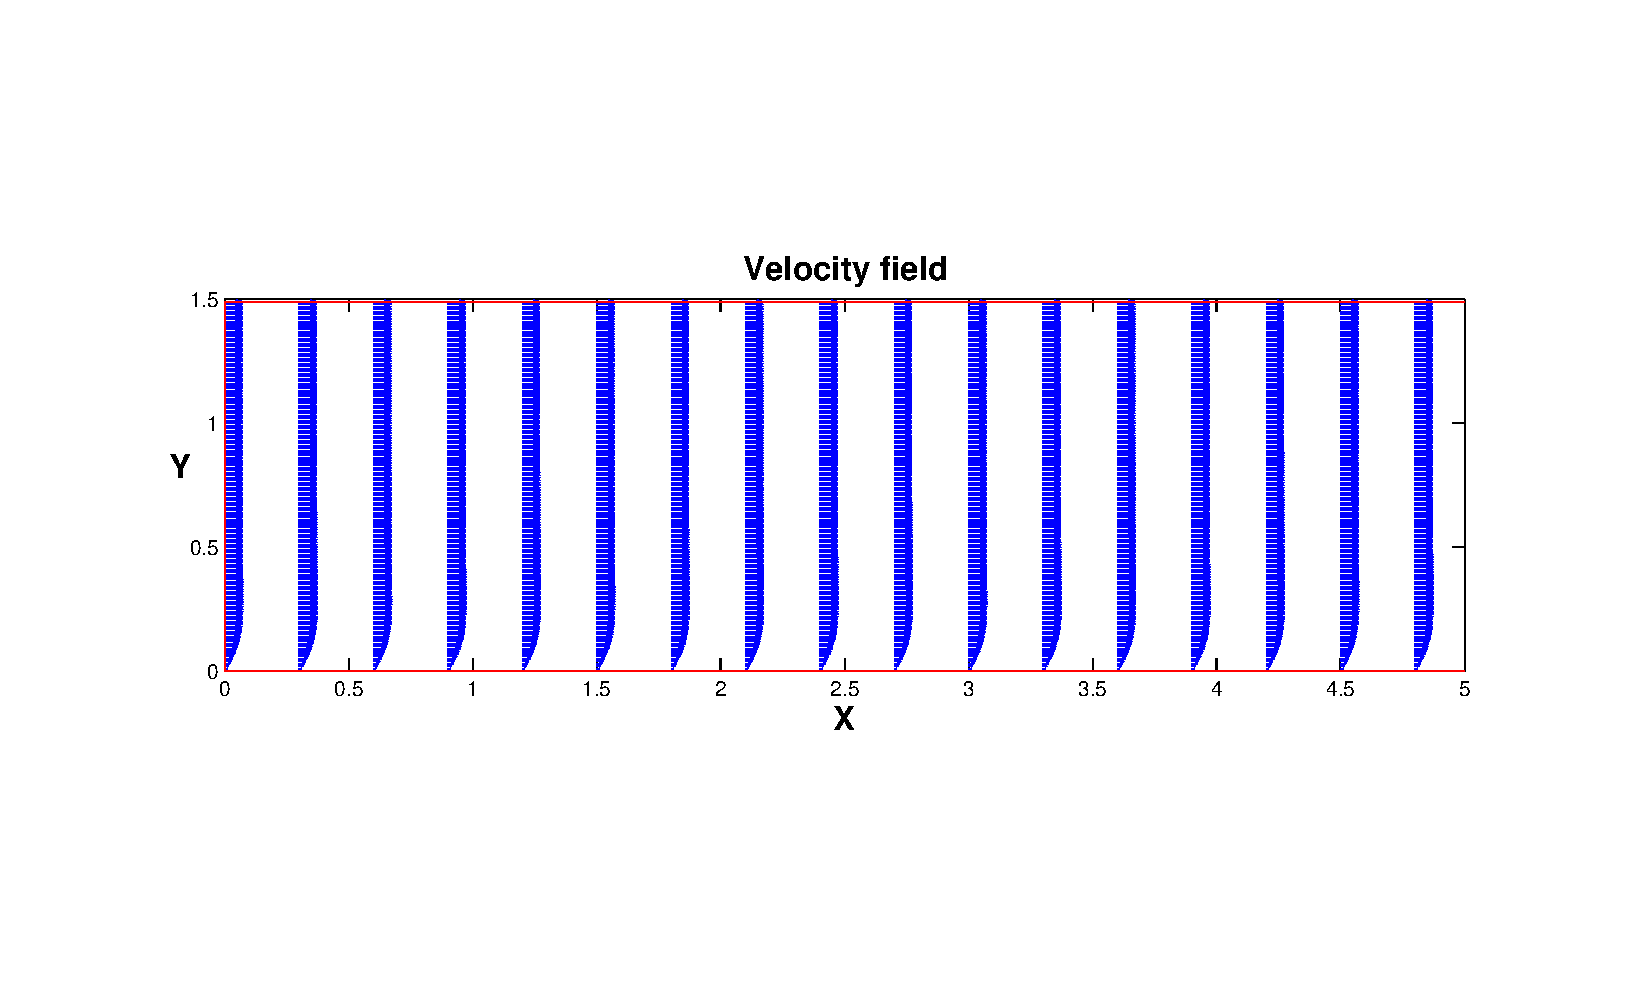
\includegraphics[scale=.4]{blasiusvp.eps}
\end{center}
\caption{Flow Between Two Parallel Plates at $Re = 500,000$}
\end{figure}

\begin{figure}
\label{blasius5}
\begin{center}
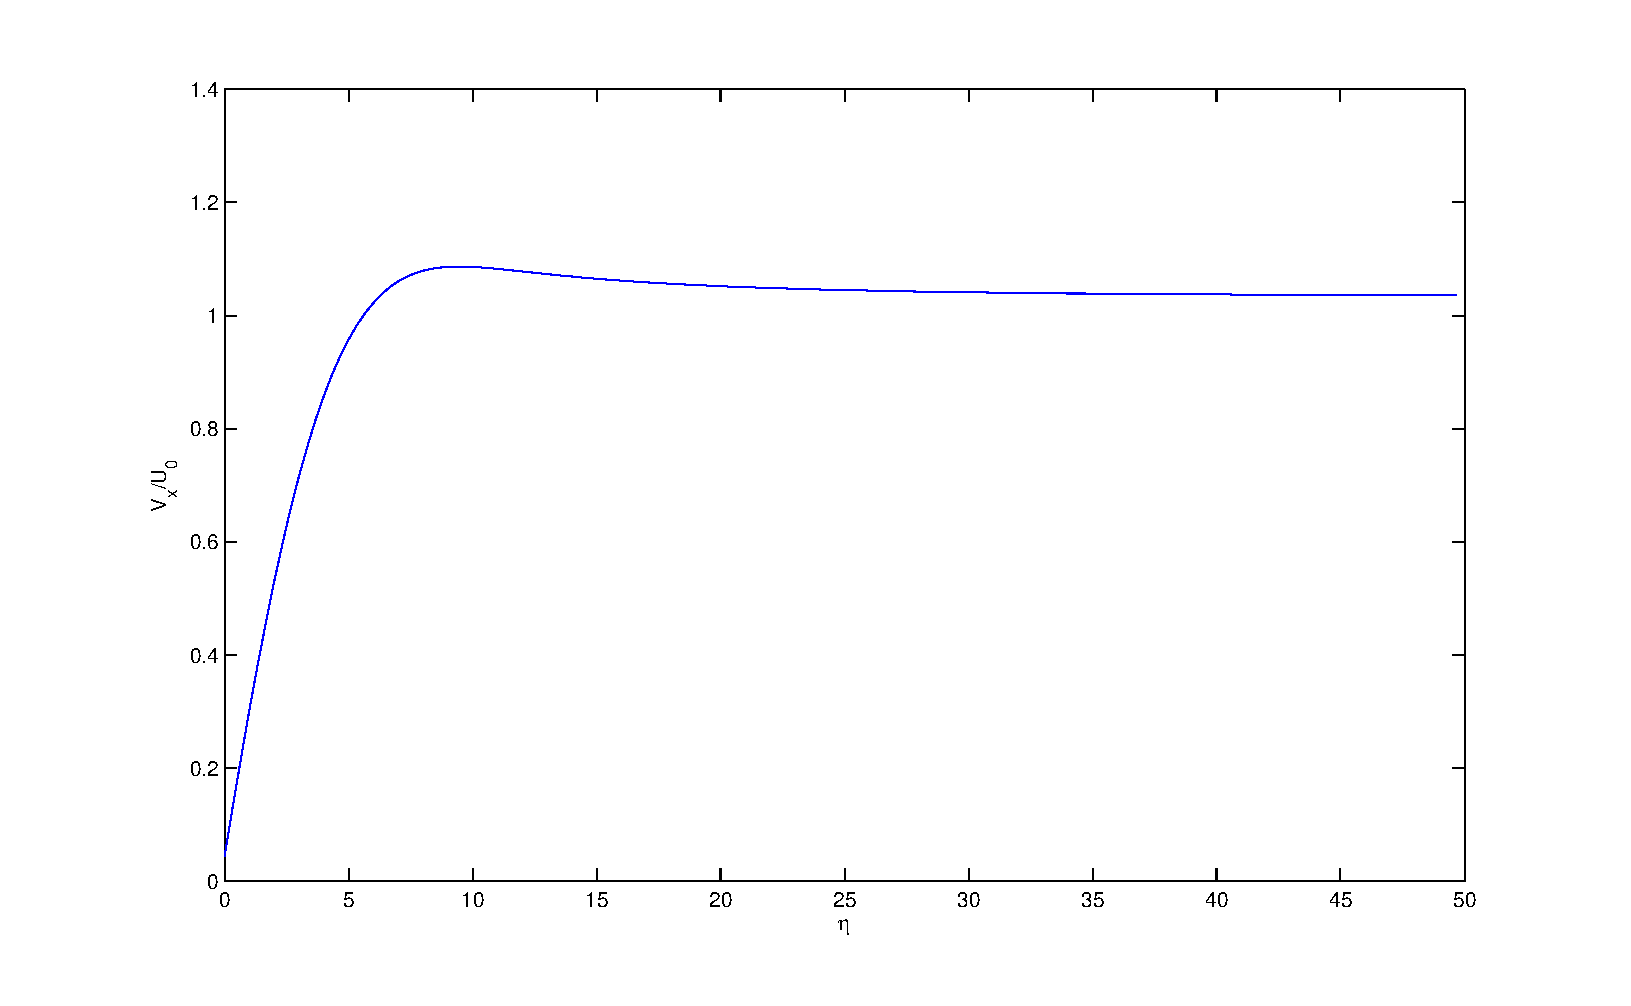
\includegraphics[scale=.4]{blasius.eps}
\end{center}
\caption{Flow Between Two Parallel Plates at $Re = 500,000$}
\end{figure}

\begin{table}
\label{table1}
\caption{Velocity in the $x$-direction vs. similarity variable at $x = 15$}
\begin{center}
\begin{tabular}{c|c}
\hline
$V_x/U_0$  &  $\eta$\\
\hline
0.044572&	0\\
0.13274	& 0.333333333\\
0.218923&	0.666666667\\
0.302261&	1\\
0.382128&	1.333333333\\
0.458035&	1.666666667\\
0.529589&	2\\
0.596505&	2.333333333\\
0.658584&	2.666666667\\
0.715718&	3\\
0.767876&	3.333333333\\
0.815102&	3.666666667\\
0.857504&	4\\
0.895244&	4.333333333\\
0.928534&	4.666666667\\
0.957621&	5\\
0.98278	& 5.333333333\\
1.004308&	5.666666667\\
1.022511&	6\\
1.037705&	6.333333333\\
1.0502	& 6.666666667\\
\hline
\end{tabular}
\end{center}
\end{table}


\section{Flow Between Two Parallel Plates}

\begin{figure}
\label{fbtpp500}
\begin{center}
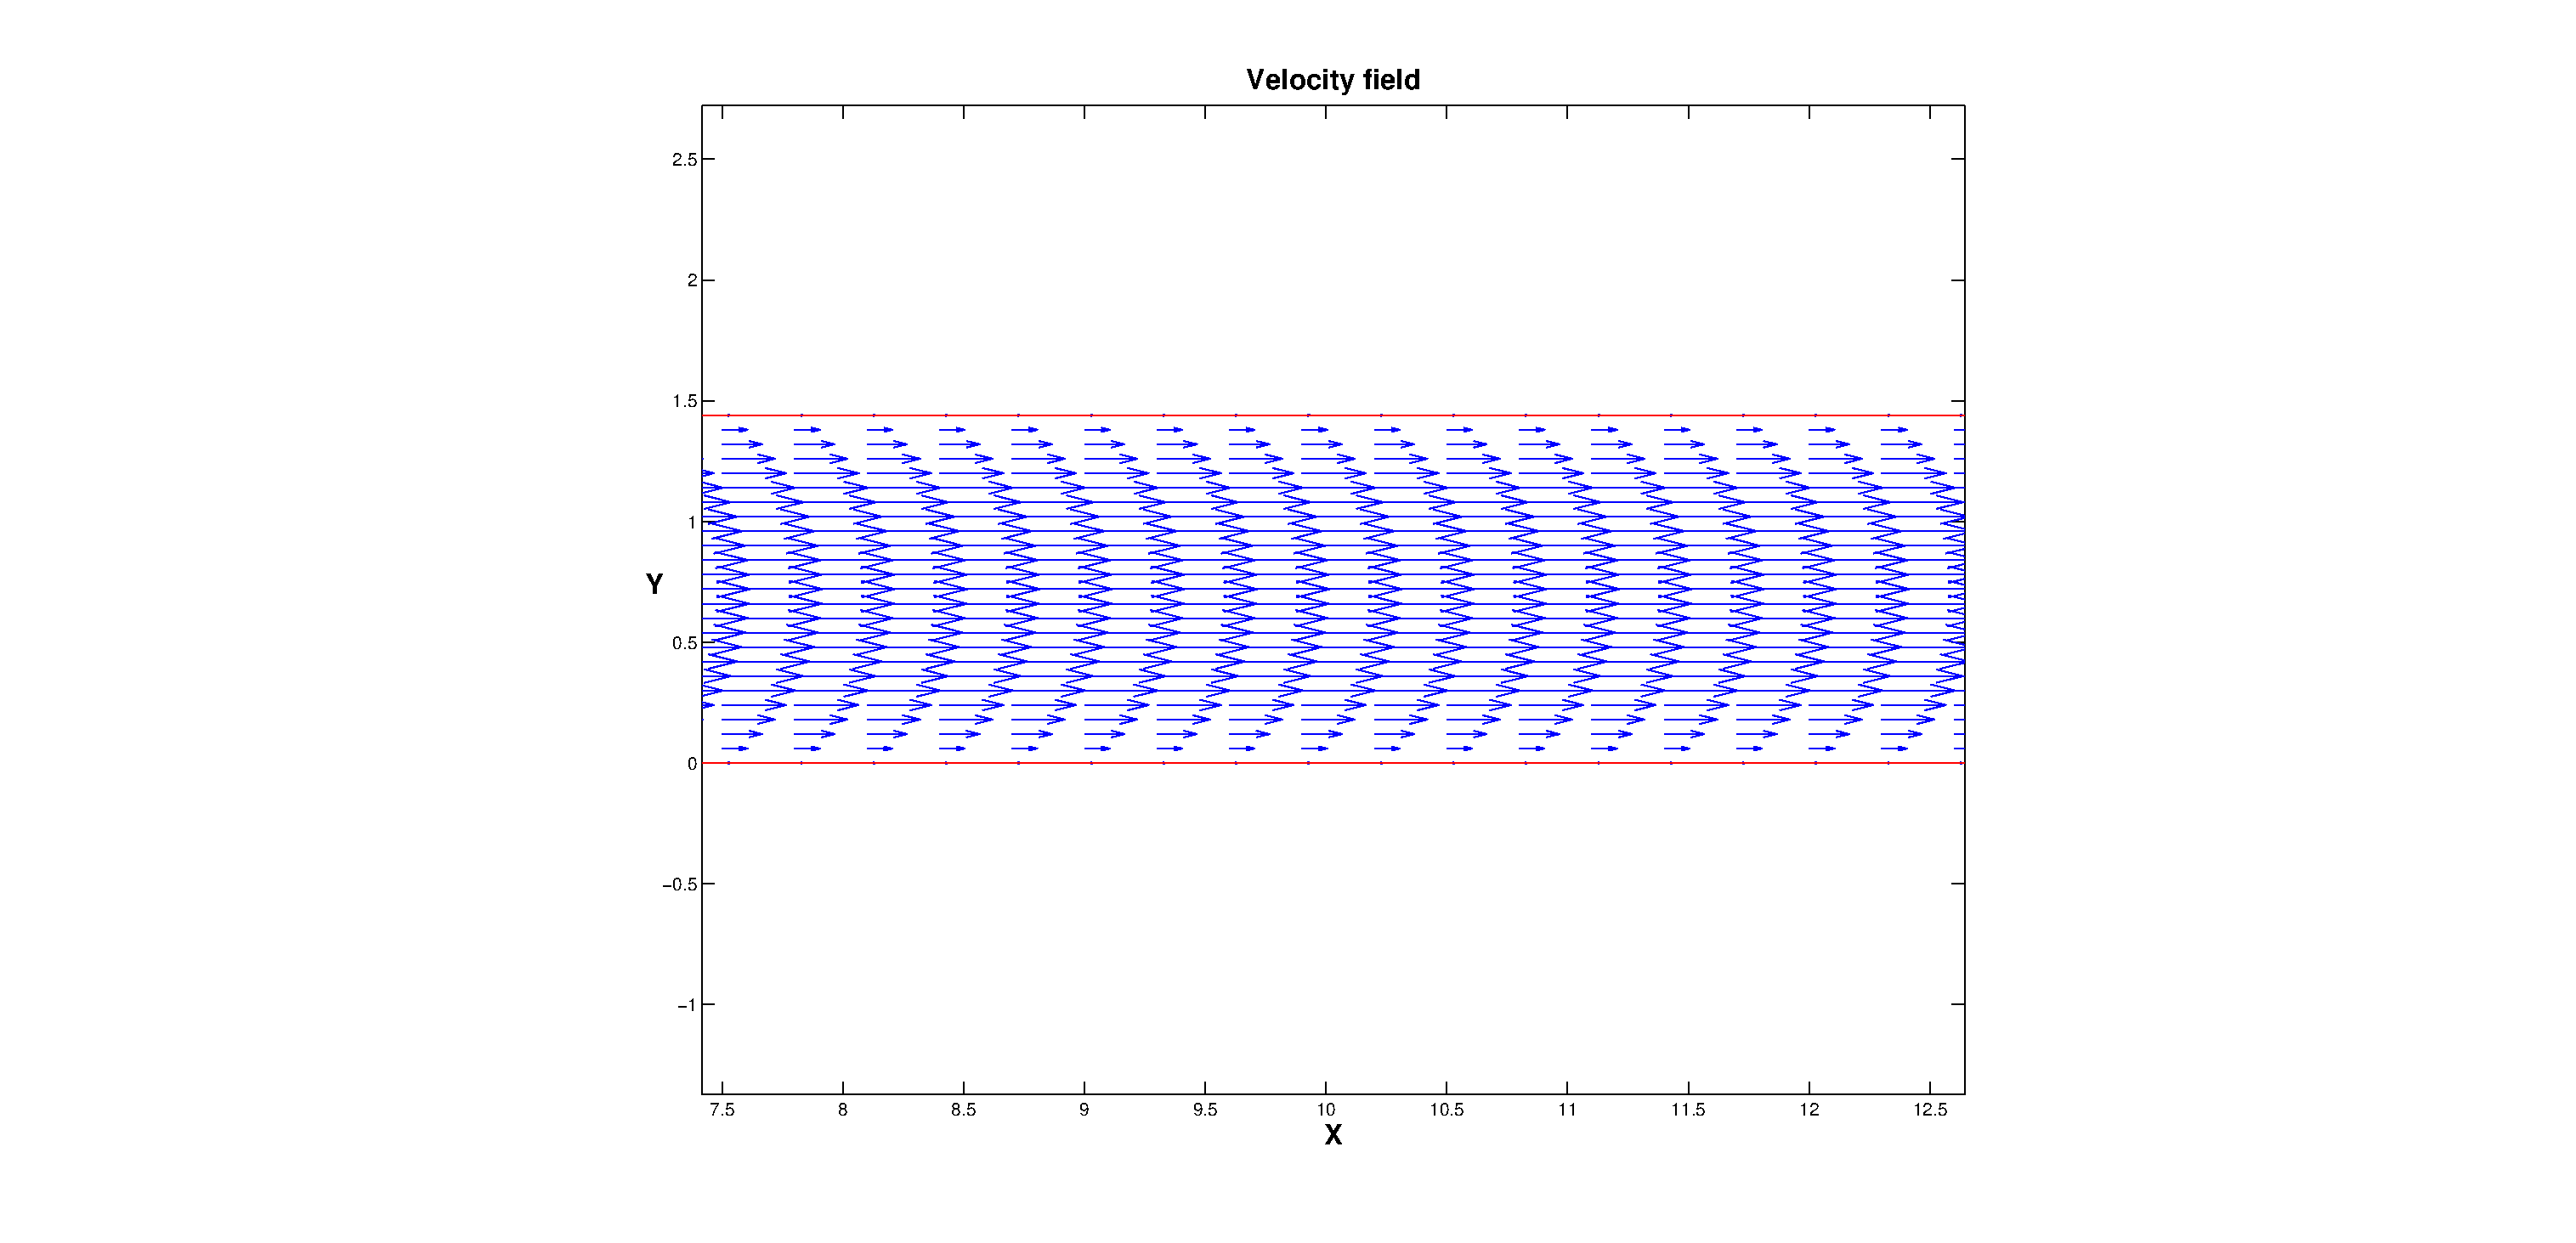
\includegraphics[scale=.3]{pplate500_velocityfield.eps}
\end{center}
\caption{Flow Between Two Parallel Plates at Re = 500}
\end{figure}

The velocity profile of a fluid flow driven by an inflow between two parallel plates is given in figure(\ref{fbtpp500}) for $Re = 500$ . We employ the same inflow velocity as before in all our simulations. In the case where $Re = 500,000$ the effect of viscosity is pronounced in a small layer close to the boundary. This small region is known as the boundary layer \cite{fmln}. Outside of this region, the flow is almost uniform.

\section{Lid-Driven Cavity Flow}

We investigate flow in a lid-driven cavity. We use the no-slip condition on the four boundaries with the lid having a constant velocity of $(1,0)$. The computational domain has dimension $1\times1$ subdivided into equally spaced subintervals in both the $x$ and $y$ directions. The Reynolds number used for this flow is $100$.  

\begin{figure}
\label{ldc1}
\begin{center}
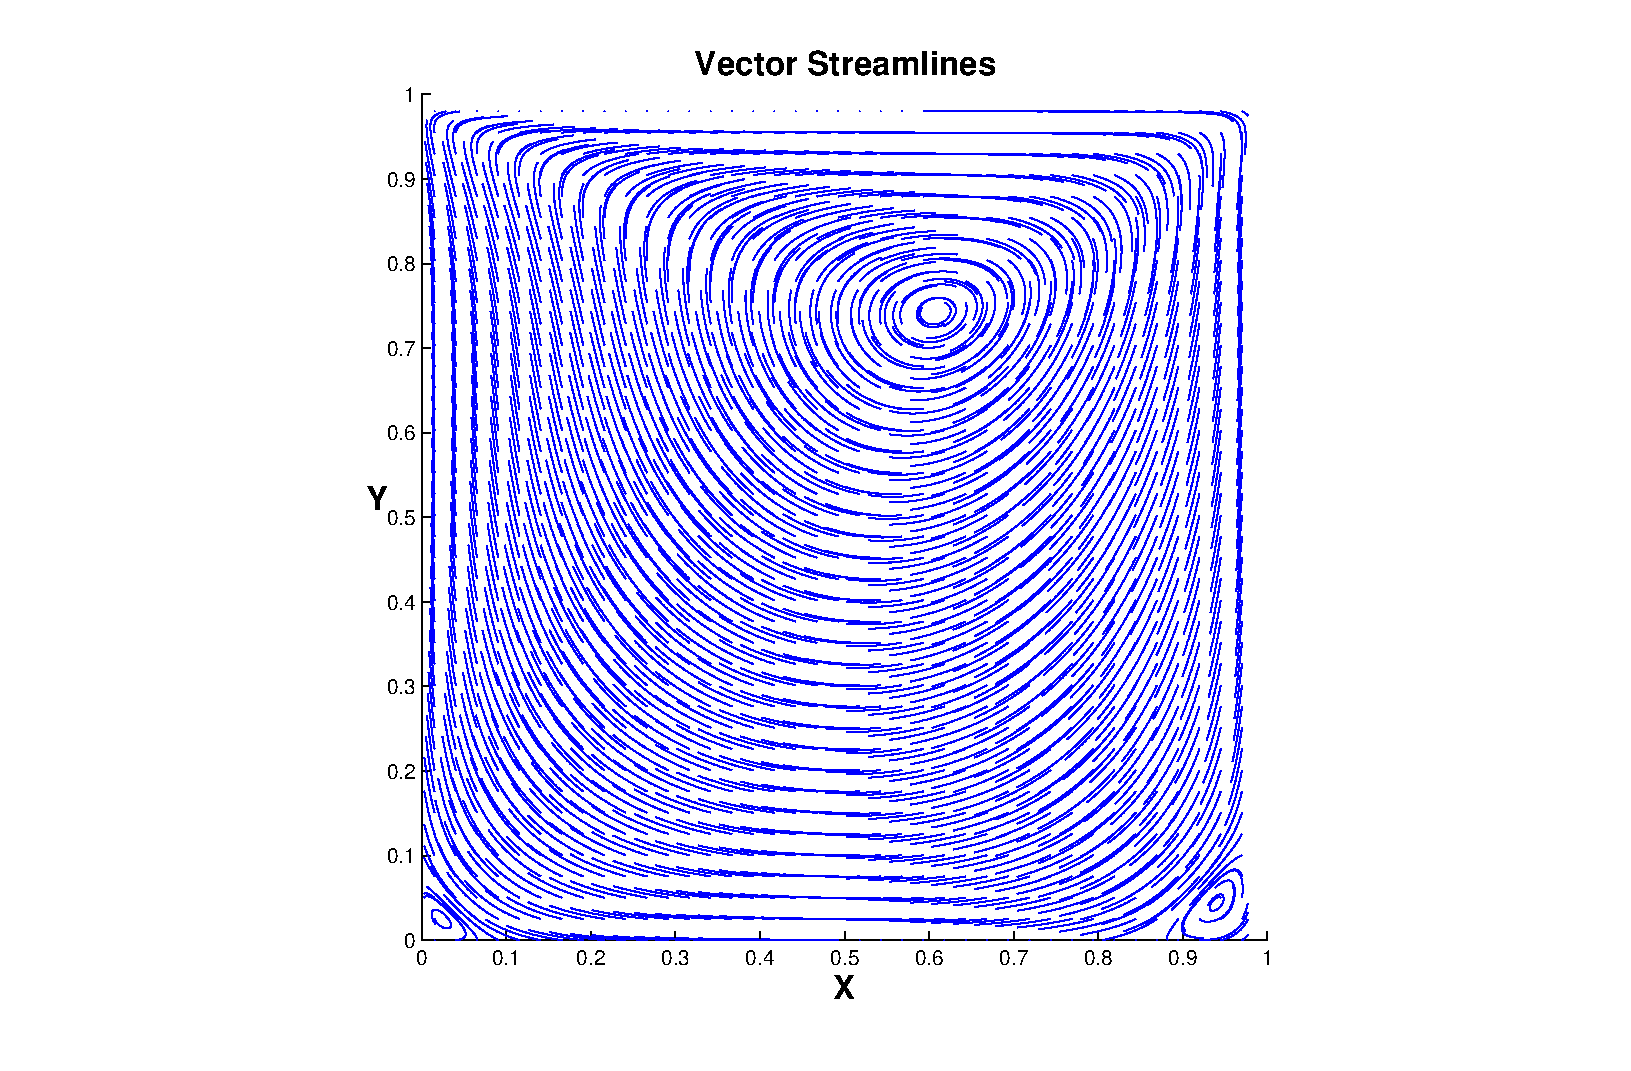
\includegraphics[scale=.5]{dcavity.eps}
\end{center}
\caption{Flow in a Lid-Driven Cavity}
\end{figure}

When the parameters are chosen as above, these regions of recirculation known as eddies are formed in the two lower corners of the cavity. 

\begin{figure}
\label{ldc2}
\begin{center}
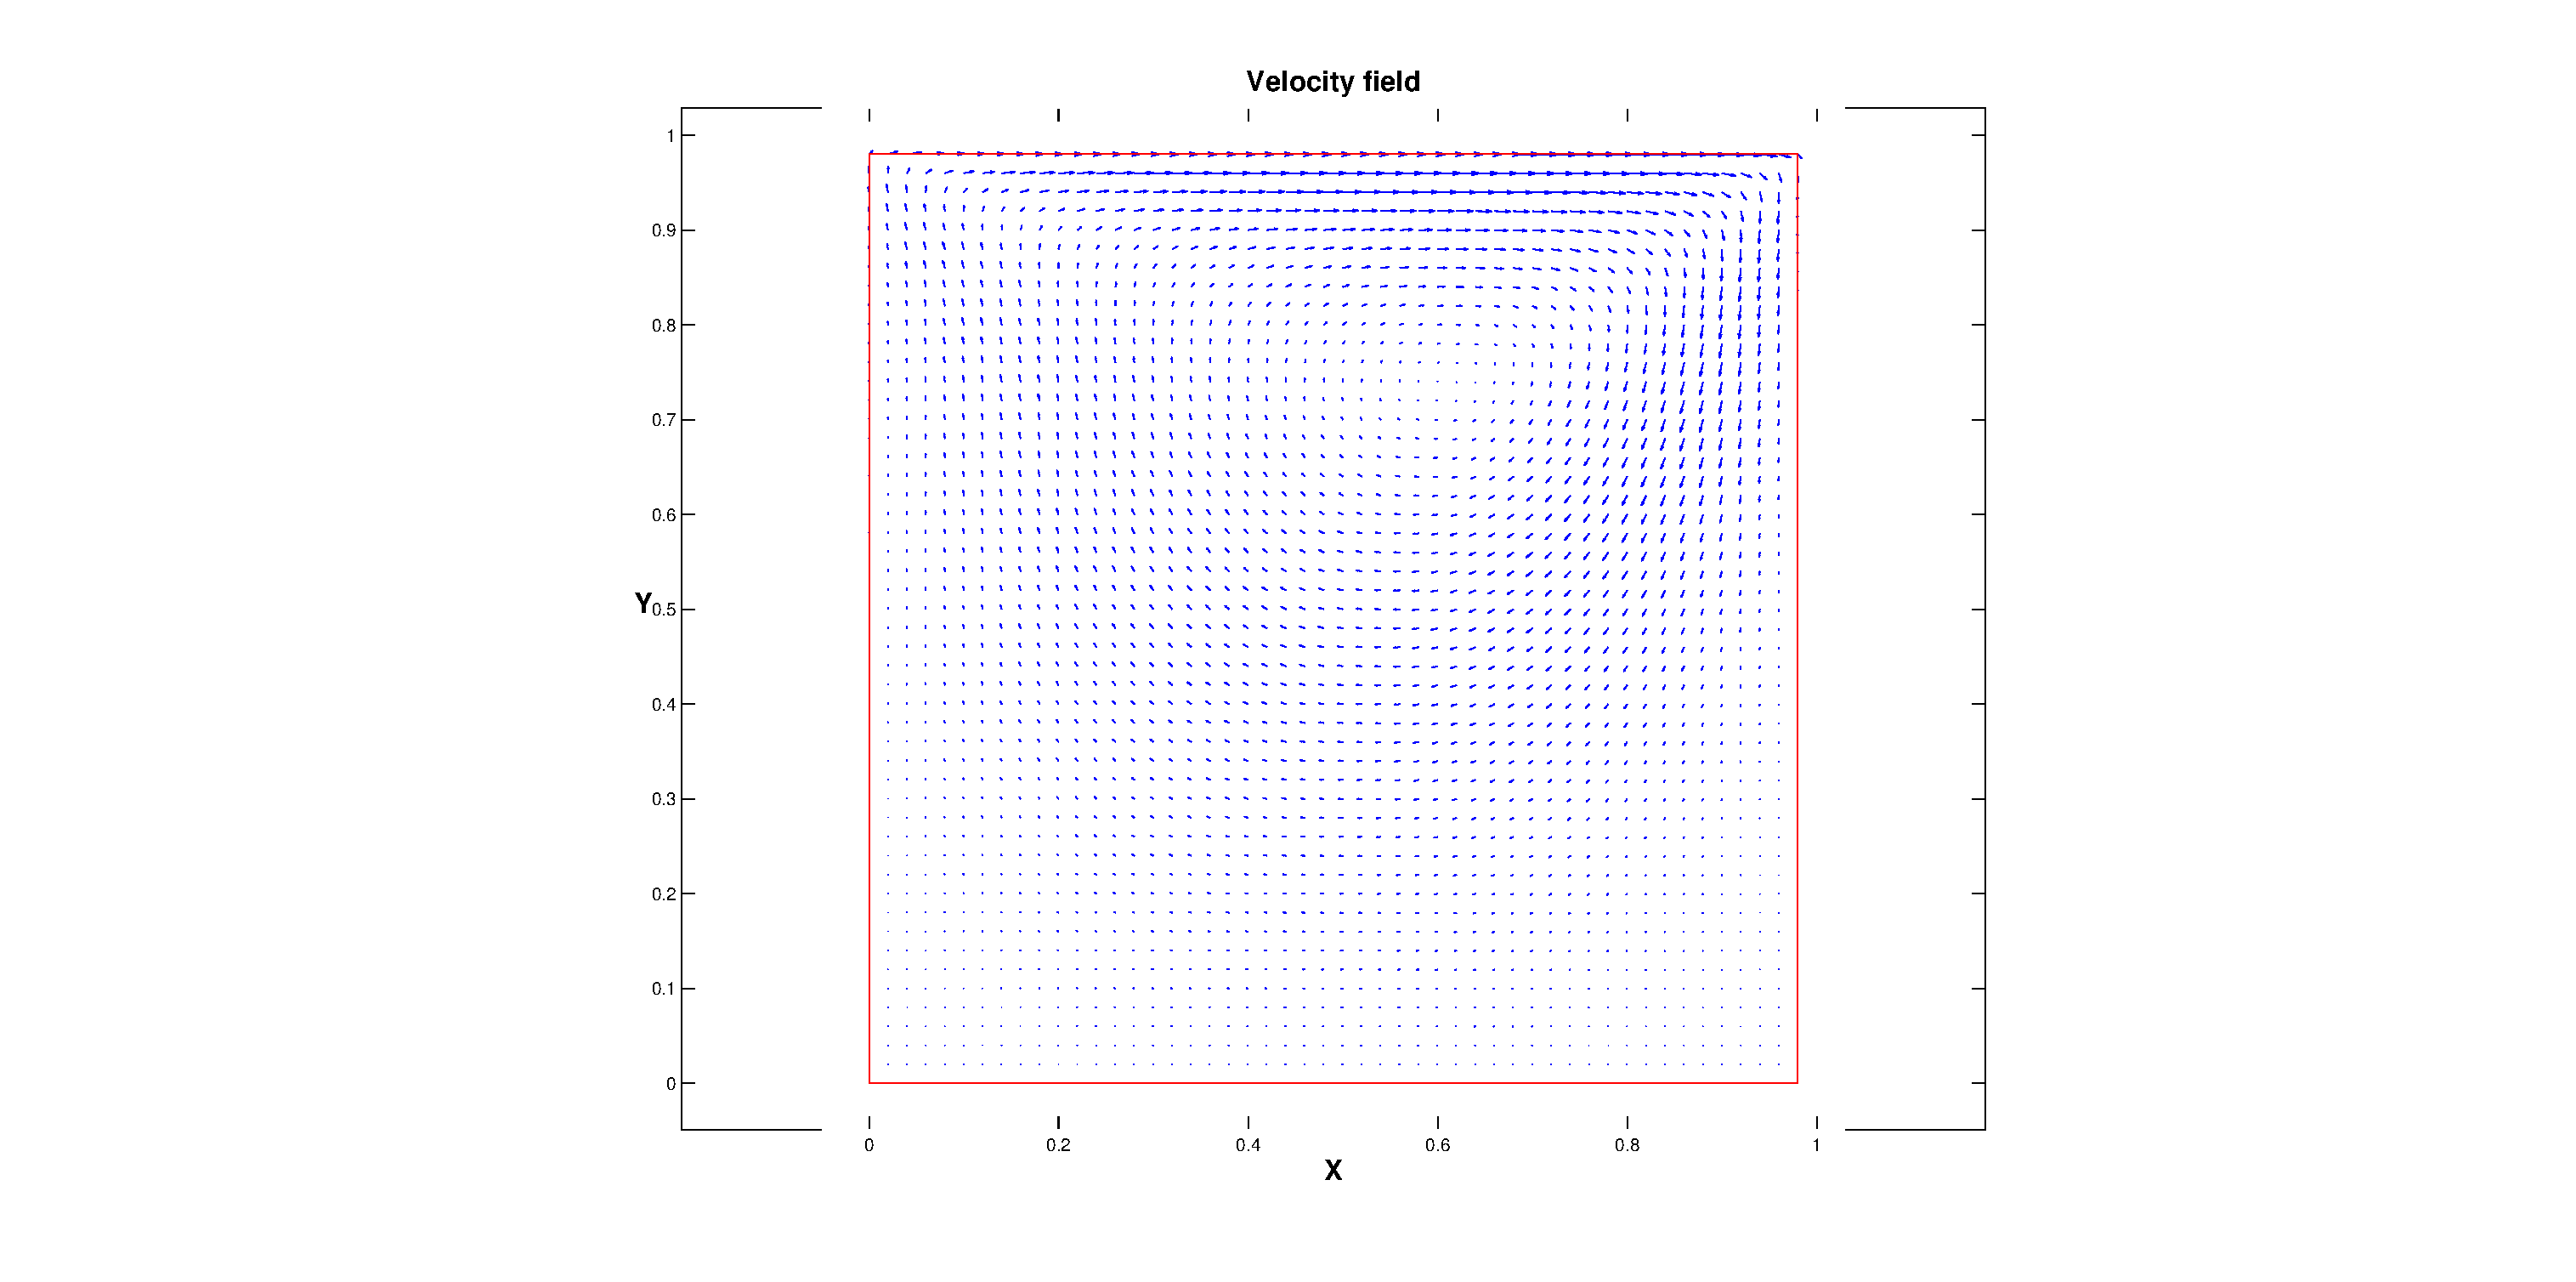
\includegraphics[scale = .3]{dcavity_velocityfield.eps}
\end{center}
\caption{Flow in a Lid-Driven Cavity}
\end{figure}

\section{Flow Over a Backward Facing Step}

We investigate flow over a backward facing step. We take the no-slip condition on the north and south boundaries and the inflow/outflow condition on the east and west boundaries. The initial inflow velocity in the horizontal direction is set to $1$ and the vertical component is set to $0$. The dimension of the domain is $30\times1.5$ in which the $x$-direction is subdivided into $100$ equally spaced subintervals and the $y$-direction is subdivided into $25$ equally spaced subintervals.The Reynolds number used for this flow is $500$. It can be seen that there is a recirculation region behind the step as one expects. 

\begin{figure}
\begin{center}
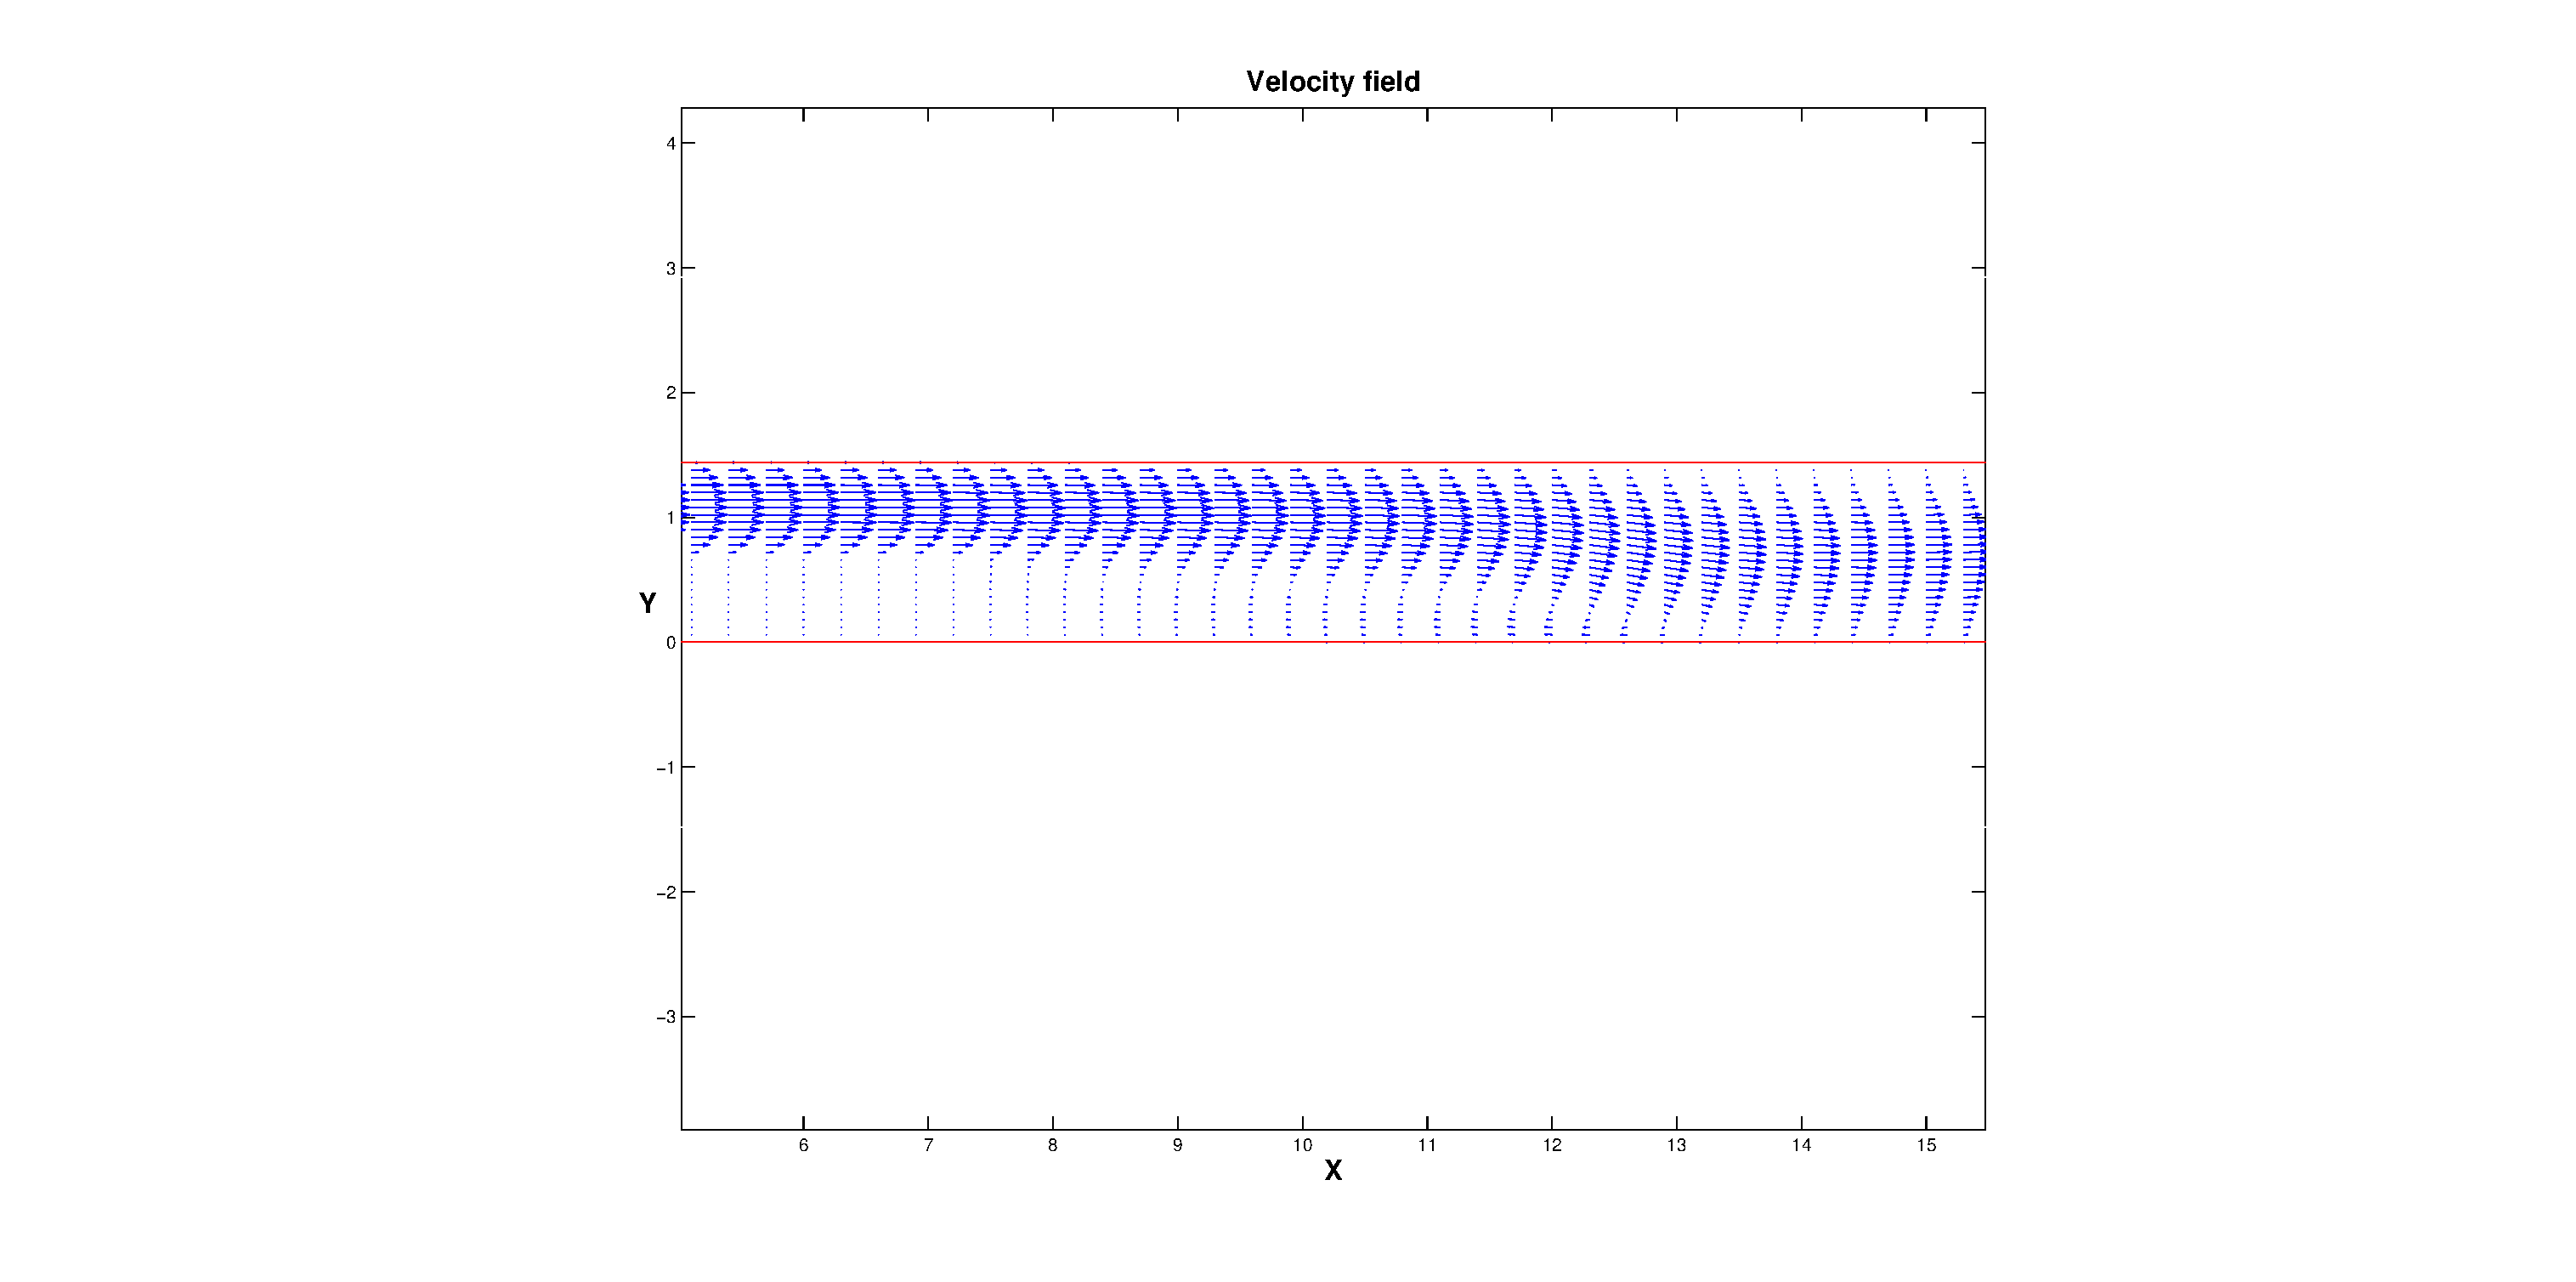
\includegraphics[scale=.3]{backstep_velocityfield.eps}
\end{center}
\caption{Flow Past a Backward Facing Step.}
\label{bwfs1}
\end{figure}

\begin{figure}
\begin{center}
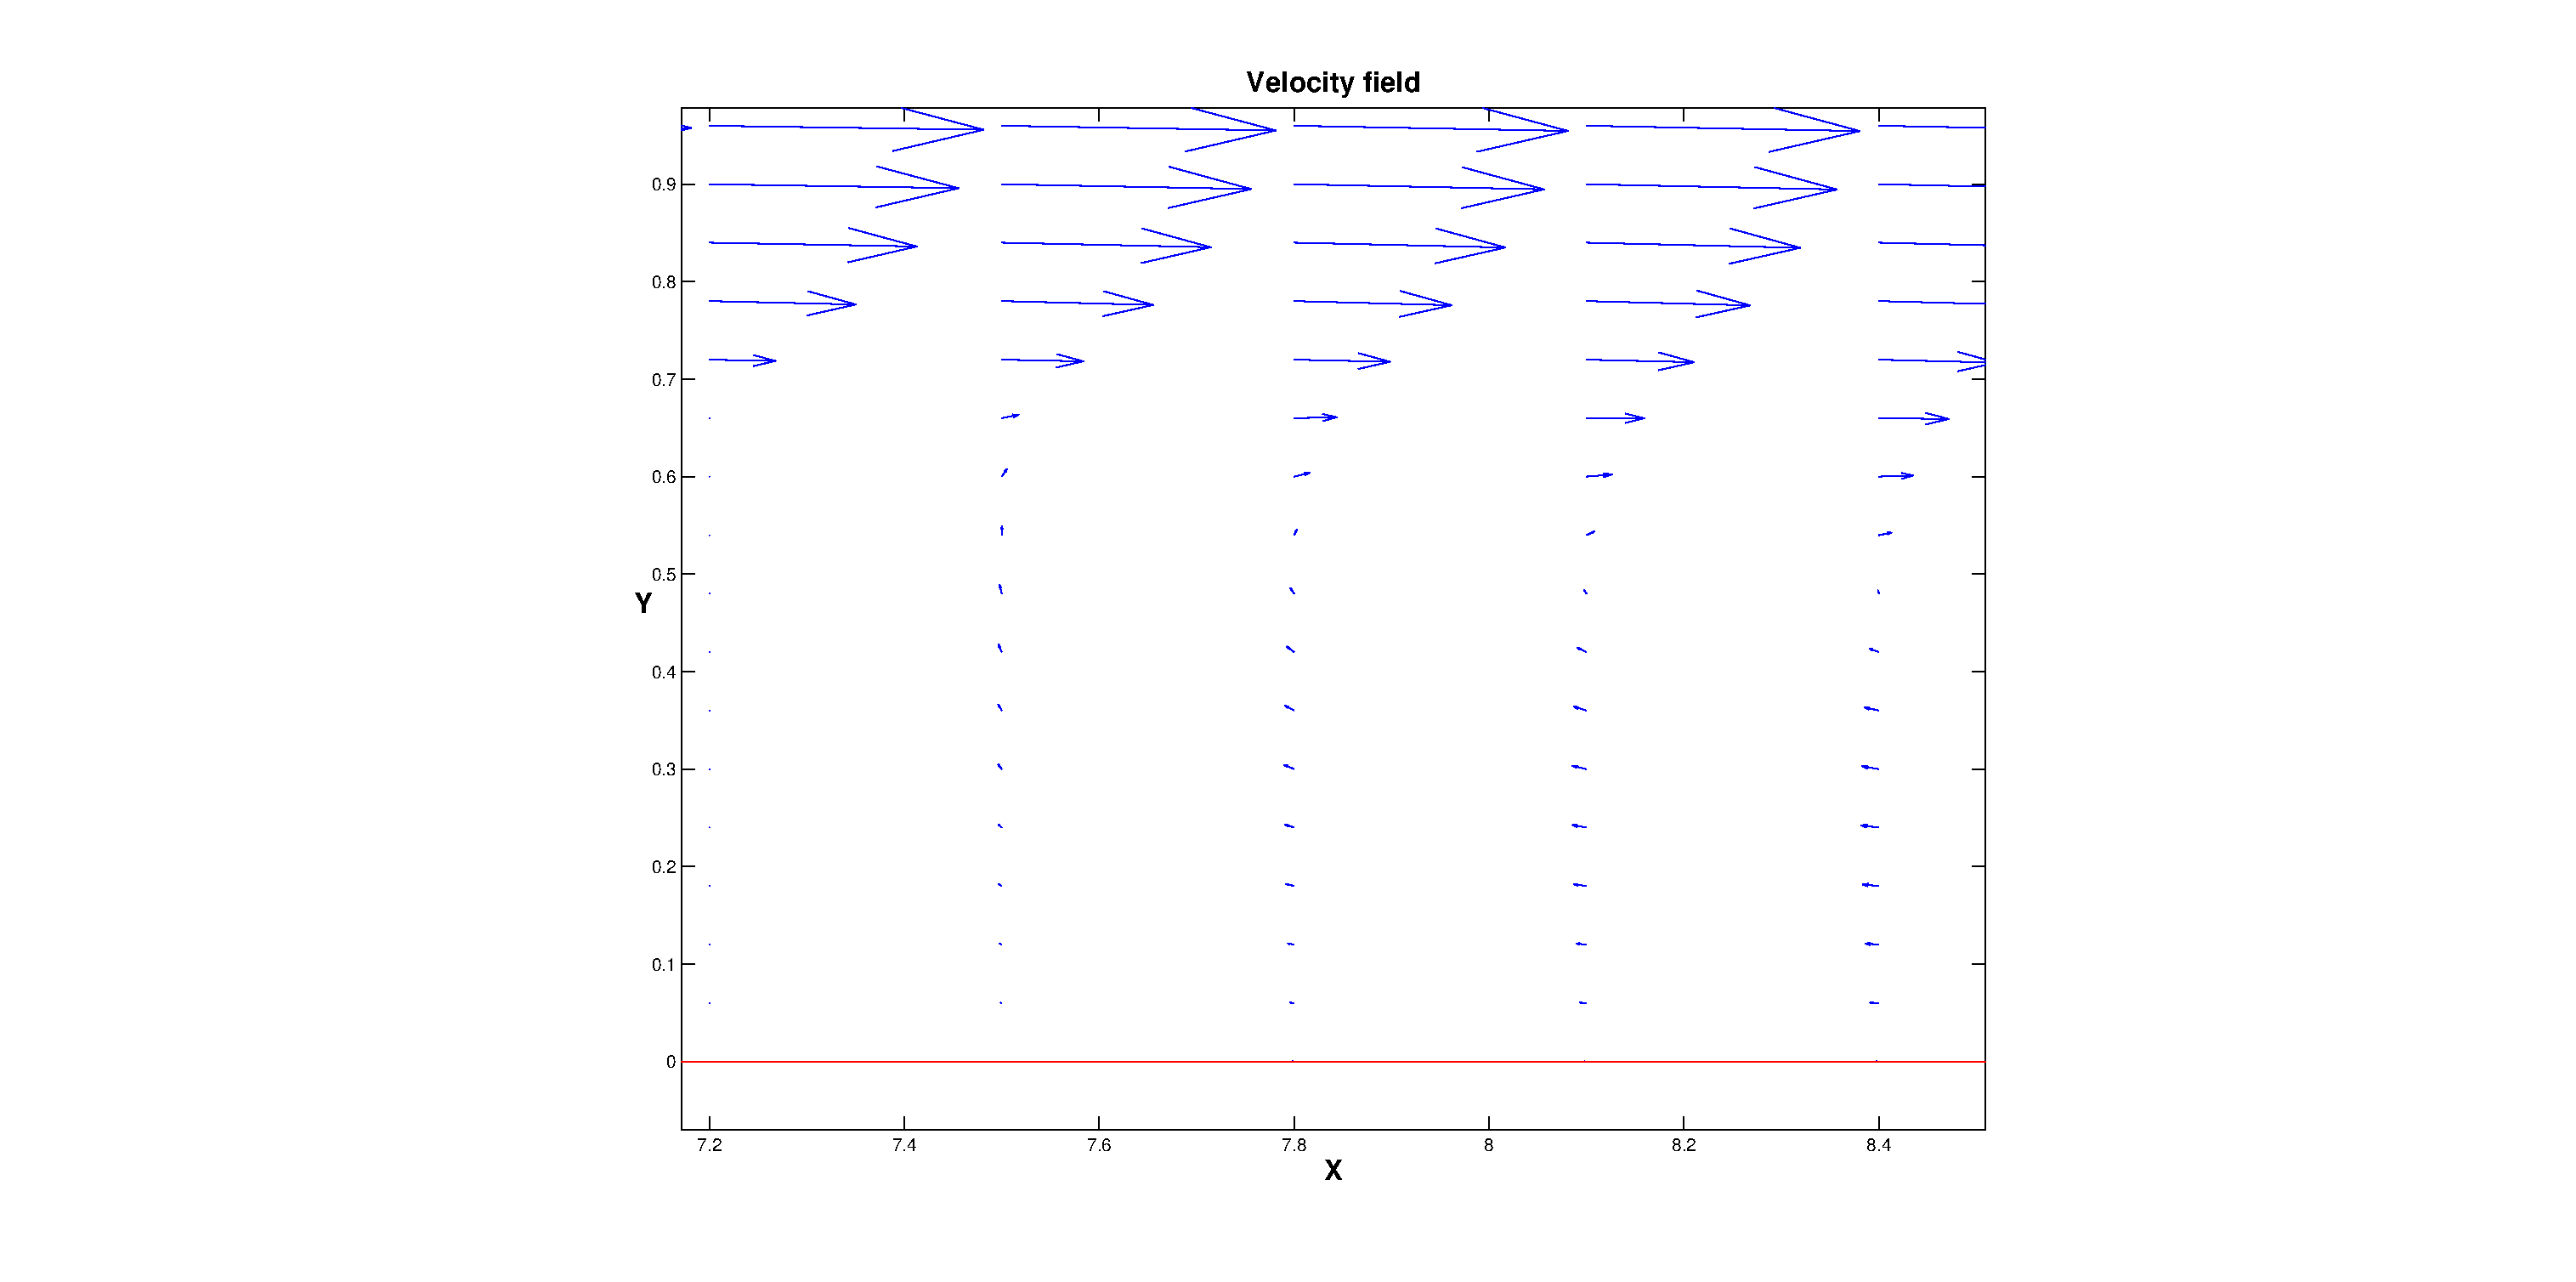
\includegraphics[scale=.3]{backstep_velocityfield1.eps}
\end{center}
\caption{Flow Past a Backward Facing Step.}
\label{bwfs2}
\end{figure}

\section{Conclusion}

In this chapter, flow between two parallel plates, flow in a lid-driven cavity, and flow over a backward facing step are investigated. The effects of different Reynold's numbers is also presented. We conclude by summarizing what has been done. 
%\end{document}
%\documentclass[12pt]{report}
%\setlength{\parindent}{0mm}
%\setlength{\parskip}{14pt}
%\renewcommand{\baselinestretch}{1.5}
%\setlength{\topmargin}{0pt}
%\setlength{\headheight}{0pt}
%\setlength{\headsep}{0pt}
%\setlength{\footskip}{45pt}
%\setlength{\textwidth}{465pt}
%\setlength{\textheight}{660pt}
%\setlength{\oddsidemargin}{10pt}
%\newcommand{\RR}{\mathrm{I\!R\!}}
%\newcommand{\FF}{\mathrm{I\!F\!}}
%\newcommand{\dt}{\frac{\partial}{\partial t}}
%\newcommand{\dq}{\frac{\partial}{\partial q }}
%\newcommand{\dr}{\frac{\partial}{\partial p }}
%\newtheorem{defi}{Definition}[chapter]
%\newtheorem{theo}{Theorem}[chapter]
%
%\begin{document}

\chapter{Summary}

In this thesis, we discussed numerical solutions of the 2-D Navier-Stokes equation. We began by laying the foundation needed for the presentation of this work. Reynold's Transport Theorem was proven and subsequently used in the derivation of the continuity equation and momentum equation from conservation of mass and linear momentum. From this point, dimensional analysis of the Navier-Stokes equations as well as the different types of boundary conditions needed in order to yeild a well-posed problem are investigated. After the completion of the derivation, we proceed to translating the continuous problem into its discrete form. In order to do this, we first introduce the concept of finite-difference approximations of continous differential operators. The Navier-Stokes equations are then discretized and a technique for handling stability issues, known as the donor-cell scheme, is presented. We also mention that other popular methods for discretizing the Navier-Stokes equations are known. For example, Finite-Volume Method and Finite-Element Method for discretization. Chorin Projection Method is also discussed for the purpose of solving the Poisson Pressure Equation that arises after discretization. In chapter 3, the functions required for implementation of the algorithm for numerically solving Navier-Stokes equations are discussed. In the fourth chapter, visualization techniques are discussed. To this end, the concept of streamlines, streaklines, and velocity profiles are presented. Finally, we present examples of classical flow problems. The problems investigated are flow between two parallel plates, flow in a lid-driven cavity, and flow past a backward facing step. It is worth mentioning that when working with the two-dimensional Navier-Stokes equations, the Stream Function-Vorticity formulation can be used to reduce the number of parameters present by eliminating the presence of the pressure term. However, in the extension to three dimensions, this effect is lost. As was stated earlier, solutions to Navier-Stokes equations are well known in 2-D but there is much left to be done in 3-D. This thesis helps to lay the foundation so the more complicated yet intersting problems can be addressed. 

%\end{document}
%\documentclass[12pt]{report}
%\usepackage{lscape}
%\setlength{\parindent}{0mm}
%\setlength{\parskip}{6pt}
%\renewcommand{\baselinestretch}{1.5}
%\setlength{\topmargin}{0pt}
%\setlength{\headheight}{0pt}
%\setlength{\headsep}{0pt}
%\setlength{\footheight}{0pt}
%\setlength{\footskip}{45pt}
%\setlength{\textwidth}{430pt}
%\setlength{\textheight}{660pt}
%\setlength{\oddsidemargin}{10pt}

%\begin{document}

\chapter*{\begin{center} References \end{center}}
\addcontentsline{toc}{chapter}{\protect\numberline{}{References}}

\begin{thebibliography}

\bibitem{cpm} [1] Chorin A J 1968 Numerical Solution of the Navier-Stokes Equations, Mathematics of Computation, Vol. 22, No. 104,745-762.

\bibitem{nsfd} [2] Griebel M, dornseifer T Neunhoeffer, T 1997 Numerical Simulation in Fluid Dynamics: A Practical Approach (Philadelphia: SIAM) 

\bibitem{ffm} [3] Munson B, Young D, Okiishi T 2008 Fundamentals of Fluid Mechanics (New York:John Wiley and Sons,Inc), Fifth Edition

\bibitem{ncse} [4] Pozrikidis C 1998 Numerical Computation in Science and Engineering (Oxford: Univ. Press)

\bibitem{feln} [5] Mason D P 1997 Finite Elasticity Lecture Notes, University of the Witwatersrand, Johannesburg, South Africa

\bibitem{fmln} [6] Mason D P 1997 Fluid Mechanics Lecture Notes, University of the Witwatersrand, Johannesburg, South Africa

%\bibitem{mpe}Chapman S 2008 Matlab Programming for Engineers Thomson, Fourth Edition

%\bibitem{wsb} http://www.worldscibooks.com/etextbook/5651/5651\underscore chap1.pdf

\end{thebibliography}
%\end{document}









\end{document}
